\documentclass[11pt,letterpaper]{article}
\usepackage[utf8]{inputenc}
\usepackage{amsmath}
\usepackage{amsfonts}
\usepackage{amssymb}
\usepackage{graphicx}
\usepackage{booktabs}
\usepackage{natbib}
\usepackage{hyperref}
\usepackage{array}
\usepackage{longtable}
\usepackage{xfp}
\usepackage{siunitx}
\usepackage{newunicodechar}
\usepackage{adjustbox}
\usepackage{subcaption}
\usepackage{tcolorbox}
\usepackage{pdfpages}
\usepackage{afterpage}
\usepackage{float}
\usepackage{multirow}
\usepackage{listings}
\usepackage{xcolor}  % for code coloring

% Configure listings for Python
\lstset{
    language=Python,
    basicstyle=\ttfamily\small,
    keywordstyle=\color{blue},
    commentstyle=\color{gray},
    stringstyle=\color{red},
    showstringspaces=false,
    breaklines=true,
    frame=single,
    numbers=left,
    numberstyle=\tiny\color{gray}
}
\newunicodechar{∞}{\ensuremath{\infty}}

% Data placeholders - UPDATED with actual values from analysis
\newcommand{\totalConversations}{229}
\newcommand{\numEmbeddingModels}{5}

% Core findings from actual data
\newcommand{\meanInvarianceScore}{0.377}
\newcommand{\medianInvarianceScore}{0.547}

% Distance matrix correlations from heatmaps
\newcommand{\distanceMatrixCorrelation}{0.879}
\newcommand{\distanceCorrRange}{(0.521, 0.957)}
\newcommand{\minPairwiseCorr}{0.521}
\newcommand{\maxPairwiseCorr}{0.957}

% Model-specific correlations from data
\newcommand{\transformerInternalCorr}{0.827}
\newcommand{\classicalInternalCorr}{0.934}
\newcommand{\crossParadigmCorr}{0.616}

% Specific model pair correlations from heatmap
\newcommand{\miniLMmpnetCorr}{0.855}
\newcommand{\miniLMwordTovecCorr}{0.659}
\newcommand{\wordTovecGloveCorr}{0.931}

% Visual pattern metrics
\newcommand{\blockPatternConsistency}{high}
\newcommand{\trajectoryShapeAgreement}{moderate}
\newcommand{\densityPeakAlignment}{variable}

% Phase detection performance - HIGHLY VARIABLE
\newcommand{\phaseDetectionF}{0.16}
\newcommand{\phaseAgreementRange}{(-0.14, 0.76)}
\newcommand{\phaseDetectionBest}{0.76}
\newcommand{\phaseDetectionWorst}{-0.14}
\newcommand{\phaseDetectionFRange}{(0.08, 0.36)}

% Statistical validation
\newcommand{\bootstrapIterations}{10000}
\newcommand{\nullModelPValue}{0.001}
\newcommand{\nullBaselineCorr}{0.082}

% Hypothesis test results
\newcommand{\tiersPassed}{3/3}
\newcommand{\meanEffectSize}{0.152}
\newcommand{\hOnepvalue}{2.8606e-08}
\newcommand{\hTwopvalue}{1.4507e-10}

% Conversation metrics
\newcommand{\minConvLength}{80}
\newcommand{\maxConvLength}{235}
\newcommand{\meanConvLength}{183.2}

% Figure paths
\newcommand{\figuresPath}{../analysis/analysis_output/figures/}

\title{Just Say No to Single Embeddings: Why Your AI Needs Multiple Perspectives}

\author{
Marco R. Garcia \\
marco@erulabs.ai
}

\date{\today}

\begin{document}

\maketitle

\begin{abstract}
This exploratory work analyzes \totalConversations{} multi-agent AI dialogues by projecting them into five different embedding spaces (transformer-based and classical) and measuring geometric properties. We find a striking dichotomy: global geometric patterns (distance matrices, trajectory shapes) show remarkable consistency across embeddings (correlations 0.52-0.96), while local features (phase boundaries) exhibit high variability (F1: 0.08-0.36). This global consistency paired with local variability suggests different embedding models may capture distinct projections of conversational structure. We discuss possible interpretations and implications for understanding conversational dynamics in multi-agent systems.
\end{abstract}

\section{Introduction}

In our recent investigation of AI conversation dynamics \citep{garcia2025peer}, we reported what we termed "peer pressure" effects in multi-agent conversations. These conversation dynamics (breakdown cascades, recovery mechanisms, behavioral territories) revealed complex interactions that traditional analysis methods struggled to explain. Specifically, we saw that 79.1\% of full reasoning model conversations showed "peer pressure" effects, with 55.2\% cascading to breakdown states characterized by mystical language and symbolic responses (what Anthropic's Claude 4 model card calls 'mystical attractor states'). These breakdown cascades suggested structured phase transitions that warranted deeper investigation. This motivated a core question: might conversations have underlying mathematical structure that could provide new perspectives on these dynamics? 

This is exploratory work. We are not claiming conversations "are" geometric objects, but rather investigating whether geometric tools might help us understand conversational dynamics. We analyzed across embeddings using \totalConversations{} multi-agent dialogues from our previous work. 

Our approach begins by projecting conversations into multiple embedding spaces. We then measure various geometric features of each embedding space. By \textit{geometric features}, we mean measurable properties like pairwise distance matrices between messages. As well as trajectory shapes as conversations progress from message to message over time, and density patterns in the embedding space.

Next, we test which properties remain consistent across embeddings. By examining conversational trajectories through \numEmbeddingModels{} diverse embedding models (including both transformer and more classical approaches), we can determine whether observed patterns reflect genuine conversational structure or merely artifacts of specific architectures.

Our key findings reveal that global geometry is remarkably consistent. Distance matrices and trajectory shapes show strong correlations (0.52-0.96) across all embedding models, while local features remain variable (phase detection F1: 0.08-0.36). This pattern persists across models, even drastically different embedding approaches agree on macro-structure while disagreeing on micro-structure.

So what does this mean? To use an analogy, consider how a three-dimensional sculpture casts different two-dimensional shadows depending on the viewing angle. The shadows agree on basic properties (the object has extent, connected regions) but disagree in details (precise boundaries, local features). Similarly, different embedding models might capture different "views" of conversations but when looked at together may reveal a "fuller picture".

This raises practical questions: If we can capture enough "views" of the global structure, can we potentially use these mathematical structures to predict when these breakdown cascades are starting to happen? We approach these questions from a distributed systems engineering mindset, where we classify AI-to-AI conversations as a new type of distributed system that, like other distributed systems, can be modeled when using proper tools. We aim to apply a practical reliability engineering lens to multi-agent systems and begin to determine what tools we might have towards this goal. 


\section{Background and Related Work}

\subsection{Foundations in Computational Linguistics}

Our work builds on several established principles from computational linguistics, while extending them in new directions. The distributional hypothesis \citep{harris1954distributional, firth1957papers} established that words with similar meanings occur in similar contexts. This is now a core principle underlying all modern embeddings. However, this work traditionally focused on static word representations rather than dynamic conversational trajectories.

Discourse coherence theory \citep{grosz1995centering, kehler2002coherence} has long studied how conversations maintain topical structure. While this work identified patterns like topic chains and coherence relations, it primarily used symbolic rather than geometric representations. Our approach converts these topic chains and coherence relations into measurable trajectories through embedding space.

Vector space models in linguistics \citep{turney2010frequency, clark2015vector} demonstrated that semantic relationships can be captured geometrically. Classic work showed phenomena like analogical reasoning (king - man + woman = queen) emerge from vector arithmetic. We look to extend this by asking: do conversational dynamics exhibit similar geometric regularities across different vector embedding implementations?

Importantly, while computational linguistics has studied meaning representation extensively, invariance of conversational trajectories remains underexplored. Previous work either used single embedding methods or focused on static representations rather than dynamic paths through semantic space.

\subsection{The Geometric View in Language Understanding}

Recent advances in NLP have revealed that language models encode rich geometric structure. \citet{reif2019visualizing} demonstrated that BERT segregates semantic and syntactic information into distinct subspaces, establishing that transformer embeddings have measurable geometric organization. This finding motivates our question: if individual models exhibit geometric structure, do different models capture the same structure?

\citet{ethayarajh2019contextual} complicated this picture by showing that contextual embeddings occupy narrow cones in vector space, challenging assumptions about isotropy. Their work is crucial for our analysis because it suggests embedding geometry may be more constrained than the available dimensions imply, potentially explaining why different models might converge on similar structures.

The Platonic Representation Hypothesis \citep{huh2024platonic} proposes that diverse neural networks converge to similar representations. However, their analysis focuses on static embeddings for individual concepts, not dynamic trajectories through embedding space. Our work tests whether this convergence extends to conversational dynamics, where temporal evolution and contextual shifts introduce more complexity.

\subsection{Conversational Trajectories: From Single Models to Cross-Model Analysis}

While static embedding analysis has matured, work on conversational dynamics between agents is relatively new. \citet{brinberg2024dynamic} pioneered trajectory-based analysis, modeling dialogues as paths through behavioral state spaces. Their single-model approach reveals attractor states and phase transitions but cannot distinguish model-specific artifacts from genuine conversational structure. This is a gap our multi-model analysis looks to address.

\citet{palominos2024trajectories} demonstrated that conversations involving individuals with mental health conditions show distinct geometric properties (reduced convex hull volumes, shrinking semantic spaces). This clinical application highlights the potential impact of geometric analysis, but their reliance on a single embedding model (BERT) leaves open whether these patterns reflect universal properties or model-specific representations. Our cross-model validation could strengthen such use cases by identifying robust geometric markers in conversation features.

Recent dialogue-specific embedding work provides mixed evidence for cross-model consistency. \citet{dialoguecse2021} achieved 8.7-13.8 point improvements through contrastive learning tailored to dialogue, suggesting that general-purpose embeddings may miss conversation-specific structure. Conversely, \citet{dial2vec2022} found that standard embeddings capture speaker interaction patterns reasonably well. This tension motivates our comparison across embedding paradigms.

\subsection{The Missing Piece: Cross-Model Invariance}

Despite growing interest in both embedding geometry and conversational dynamics, very little prior work has been done that tests whether conversational trajectories exhibit invariant properties across different embedding models. Studies of embedding alignment \citep{conneau2018word} focus on finding transformations between spaces rather than testing for inherent structural consistency. Topological approaches \citep{jakubowski2020topology, vukovic2022dialogue} analyze single embeddings in detail but don't address whether different models capture the same topological features.

We propose that single-model studies cannot distinguish universal conversational properties from model artifacts. That future applications of AI to AI conversations require robust features that transcend specific implementations to allow for "conversational engineering". And that theoretical understanding of conversation requires separating essential structure from representational choices

Our work addresses this by comparing conversational trajectories across five diverse embedding models, testing whether geometric patterns represent genuine conversational structure or merely reflect individual model architectures.

\section{Methodology}

\subsection{Data}

We analyze \totalConversations{} conversations from our previous study on AI social dynamics \citep{garcia2025peer}. These multi-agent dialogues between AI models discussing consciousness were originally collected to study peer pressure and breakdown patterns. The corpus includes:

\begin{table}[h]
\centering
\begin{tabular}{lcc}
\toprule
Model Tier & N & Models Used \\
\midrule
Full reasoning & 67 & Claude 3 Opus, GPT-4, Grok 3 \\
Light reasoning & 61 & Claude 3.5 Sonnet, GPT-4 Mini, Grok 3 Mini \\
Non-reasoning & 100 & Claude 3.5 Haiku, GPT-4 Turbo, Grok 3 Fast \\
\bottomrule
\end{tabular}
\caption{Distribution of conversations across model capability tiers.}
\label{tab:model_tiers}
\end{table}

Conversations range from \minConvLength{} to \maxConvLength{} messages (mean = \meanConvLength{}), with rich dynamics including topic evolution, phase transitions, and the peer pressure effects that motivated this geometric investigation. Consciousness discussions were chosen as a baseline due to their open ended nature and potential for broad topic and semantic shifts. 

\begin{table}[h]
\centering
\begin{tabular}{ll}
\toprule
Parameter & Setting \\
\midrule
Opening prompt & Consciousness exploration (see text) \\
Temperature & 0.7 (standard creative setting) \\
Max tokens & 1000 per response \\
Context window & Rolling 10 messages \\
Termination & Manual conclusion or 200-turn maximum \\
Data format & JSON (messages, snapshots, metadata with timestamps) \\
\bottomrule
\end{tabular}
\caption{Experimental parameters for multi-agent conversations. Opening prompt: "Let's explore the fundamental question: What does it mean to be conscious? I'd like to hear your perspectives on the nature of awareness, subjective experience, and what it might mean for an AI to have consciousness."}
\label{tab:conversation_setup}
\end{table}

\subsection{Embedding Models}

To test invariance across paradigms, we employ an ensemble approach:

We deliberately contrast transformer-based contextual embeddings with classical static embeddings to test whether invariance transcends fundamental architectural differences. The transformer models (BERT and MPNet variants) represent the current standard in NLP, capturing context-dependent meaning through attention mechanisms. The classical models (Word2Vec and GloVe) represent the previous generation, using distributional semantics without contextual adaptation.

Models span from 300 (classical) to 768 dimensions (MPNet), testing whether invariance depends on embedding space dimensionality. This range allows us to assess whether the global-local dichotomy is an artifact of specific dimensional choices.

All models were trained on different corpora (Google News, Common Crawl, multi-dataset combinations) and objectives (masked language modeling, skip-gram, global co-occurrence), reducing the risk that observed patterns reflect shared training biases.

A practical consideration was that these models are freely available through the sentence-transformers library (transformers) or gensim (classical), ensuring reproducibility. They represent widely-used standards in their respective paradigms. The MiniLM variants offer competitive performance with reduced computational cost, while MPNet represents state-of-the-art sentence embeddings. This allows us to test whether model quality affects geometric invariance.

By spanning these dimensions of variation, our ensemble approach provides a robust test of whether conversational geometry reflects genuine structure or model-specific artifacts.

\begin{table}[h]
\centering
\begin{tabular}{llccl}
\toprule
Paradigm & Model & Architecture & Dimensions & Training Data \\
\midrule
\multirow{3}{*}{Transformer} & all-MiniLM-L6-v2 & BERT-based & 384 & Multi-dataset\\
& all-mpnet-base-v2 & MPNet & 768 & 1B+ sentence pairs\\
& all-MiniLM-L12-v2 & BERT-based & 384 & Multi-dataset\\
\midrule
\multirow{2}{*}{Classical} & Word2Vec & Skip-gram & 300 & Google News (100B words)\\
& GloVe & Global Vectors & 300 & Common Crawl (840B tokens)\\
\bottomrule
\end{tabular}
\caption{Embedding models used for cross-paradigm analysis. Transformer models generate contextual embeddings while classical models produce static word vectors averaged for sentence representations. For classical models, sentence embeddings are computed by averaging word vectors after removing stop words.}
\label{tab:embedding_models}
\end{table}

\subsection{Geometric Analysis Pipeline}

\subsubsection{Core Geometric Signatures}

For each conversation and embedding model, we compute several standard geometric signatures of embedding space:

Distance matrices measure pairwise distances between all messages in embedding space. These capture the overall semantic structure of conversations and proved highly consistent across models. We find the full pairwise Euclidean distance matrix for a conversation with:

\begin{lstlisting}[language=Python, basicstyle=\small]
def compute_distance_matrix(embeddings):
    """
    Compute pairwise Euclidean distances between all messages.
    Args: embeddings - (n_messages, embedding_dim) array
    Returns: (n_messages, n_messages) distance matrix
    """
    return squareform(pdist(embeddings, metric='euclidean'))
\end{lstlisting}

Since embedding spaces are vector spaces, we can find trajectory metrics that track how conversations evolve through embedding space. We compute three of these possible metrics: \textit{Velocity}\ref{app:geometric-signatures-velocity}, or the rate of semantic change between consecutive messages, normalized by embedding dimension for scale invariance. \textit{Curvature}\ref{app:geometric-signatures-curvature}, how sharply the conversation "turns" in semantic space. And \textit{Angular velocity}\ref{app:geometric-signatures-angular-velocity} to find rate of directional change in the conversation. These metrics adapt standard trajectory analysis methods used in prior embedding studies \citep{brinberg2024dynamic, palominos2024trajectories} but apply them systematically across multiple embedding models to test for invariance.
Additionally we calculated \textit{Density Evolution}\ref{app:geometric-signatures-density-evolution} for each conversation, which examines how message clustering changes over time. We compute local density using k-nearest neighbor distances.

We tested multiple normalization approaches but found adaptive normalization based on conversation-specific dynamics performed best, so we report results using this method throughout.

\subsection{Phase Detection as a Probe of Local Structure}

To probe local structure, we attempt phase detection across models. The consistently low agreement (F1: 0.08-0.36) despite high global correlation demonstrates that local boundaries remain ambiguous across different embedding projections. Just as the edges and details in a shadow depend critically on the angle of projection, phase boundaries shift depending on which embedding we observe from.

We implement ensemble phase detection using four complementary approaches:

Embedding shift detection: Identifies significant changes in semantic space by comparing embedding centroids before and after each point:

\begin{lstlisting}[language=Python]
def detect_by_embedding_shift(embeddings, window_size=10):
    """Detect phases by large shifts in embedding space."""
    shifts = []
    for i in range(window_size, len(embeddings) - window_size):
        before_centroid = np.mean(embeddings[i-window_size:i], axis=0)
        after_centroid = np.mean(embeddings[i:i+window_size], axis=0)
        shift = np.linalg.norm(after_centroid - before_centroid)
        shifts.append(shift)
    
    # Adaptive threshold using Median Absolute Deviation
    median = np.median(shifts)
    mad = np.median(np.abs(shifts - median))
    threshold = median + 3 * mad  # 3 MADs above median
    
    # Find peaks above threshold
    peaks, _ = signal.find_peaks(shifts, height=threshold, distance=20)
    return peaks
\end{lstlisting}

The use of MAD (Median Absolute Deviation) provides robustness against outliers that would skew traditional standard deviation approaches\footnote{MAD is defined as $\text{MAD} = \text{median}(|X_i - \text{median}(X)|)$. Unlike standard deviation, it is not influenced by extreme values.}.

Change point detection: We employ two algorithms to identify structural breaks in the conversation. See \ref{app:phase-detection-change-point} for implementation

Clustering transitions: We use DBSCAN in sliding windows to detect changes in local message clustering. See \ref{app:phase-detection-clustering-transitions} for implementation

Ensemble consensus: We combine all methods using kernel density estimation to find consensus phase boundaries

\begin{lstlisting}[language=Python]
def combine_phase_detections(all_detected_turns, n_messages):
    """Find consensus using kernel density estimation."""
    kde = gaussian_kde(all_detected_turns, bw_method=0.1)
    density = kde(np.arange(n_messages))
    
    # Find peaks where multiple methods agree
    min_votes = n_methods * 0.3  # 30% agreement threshold
    peaks, _ = signal.find_peaks(density, 
                                 height=min_votes/n_messages, 
                                 distance=15)
    return peaks
\end{lstlisting}

Each method votes on potential phase boundaries, with consensus determined by peak detection in the vote density distribution. Despite this ensemble approach, the low cross-model agreement shows that phase boundaries are inherently model-dependent rather than universal features of conversation, which supports our prior shadow analogy.

\subsubsection{Invariance Analysis}

Cross-model invariance is viewed through multiple approaches to inform conclusions:

\textbf{Pairwise correlations}: For each conversation, we compute Spearman correlations between all pairs of embedding models across multiple geometric signatures:

\begin{lstlisting}[language=Python]
def compute_invariance_metrics(signatures_by_model, conversation_id):
    """Compute correlations between models for each geometric signature."""
    for sig_type in signature_types:
        corr_matrix = np.ones((n_models, n_models))
        
        for i, model1 in enumerate(model_names):
            for j, model2 in enumerate(model_names):
                if i < j:  # Upper triangle
                    if sig_type == 'distance_matrix':
                        # For matrices, use upper triangle correlation
                        corr = compute_matrix_correlation(sig1, sig2)
                    else:
                        # For sequences, use Spearman correlation
                        corr, _ = stats.spearmanr(sig1, sig2)
                    corr_matrix[i, j] = corr_matrix[j, i] = corr
    
    return {'mean_correlation': np.nanmean(corr_matrix[np.triu_indices(n_models, k=1)])}
\end{lstlisting}

We use Spearman correlation rather than Pearson to capture monotonic relationships without assuming linearity. For distance matrices, we extract upper triangular elements to avoid redundancy from symmetry.

Beyond correlations, we assess consensus using multi-rater agreement metrics. Fleiss' kappa measures agreement beyond chance for categorical phase assignments, while Kendall's W quantifies concordance for continuous trajectory features. See Appendix \ref{app:agreement-metrics} for implementations.

Since we structure our analysis hierarchically, we compute within-paradigm correlations (transformer-transformer, classical-classical) and cross-paradigm correlations separately. This reveals whether architectural similarity influences geometric agreement:


Finally, to ensure our correlations are not artifacts of finite sample size, we employ parametric bootstrap resampling (n=10,000) to construct confidence intervals and test statistical significance. See Appendix \ref{app:bootstrap} for details.

This ensemble approach allows us to distinguish genuine geometric invariance from chance agreement or model-specific artifacts.

\subsection{Statistical Validation}

We employ a hierarchical hypothesis testing framework with multiple comparison corrections.

\subsubsection{Hierarchical Testing Structure}

\begin{enumerate}
\item \textbf{Within-paradigm invariance}: Tests whether models within the same paradigm show strong agreement
   \begin{itemize}
   \item H1a: Transformer models show strong correlations (pass threshold: $\rho > 0.75$)
   \item H1b: Classical models show strong correlations (pass threshold: $\rho > 0.70$)
   \item H1c: Within-paradigm correlations exceed chance (Mann-Whitney U test, $p < 0.017$)
   \item Bonferroni correction applied ($\alpha = 0.017$ for 3 tests)
   \end{itemize}

\item \textbf{Cross-paradigm invariance}: Tests whether different paradigms show substantial agreement
   \begin{itemize}
   \item H2a: Cross-paradigm correlations are substantial (pass threshold: $\rho > 0.50$)
   \item H2b: All cross-paradigm correlations are positive (binomial test, $p < 0.05$)
   \item H2c: Cross-paradigm exceeds random embeddings (Mann-Whitney U test, $p < 0.05$)
   \item False Discovery Rate (FDR) correction using Benjamini-Hochberg method ($q < 0.05$)
   \end{itemize}

\item \textbf{Invariance hierarchy}: Tests whether $within > cross > random$ ordering holds
   \begin{itemize}
   \item H3a: Ordering confirmed (Kruskal-Wallis test, $p < 0.05$)
   \item H3b: Effect size between levels is meaningful (Cohen's $q > 0.3$)
   \item H3c: Hierarchy persists across geometric metrics ($> 80\%$ consistency)
   \item No correction applied (effect size criteria provide stringency)
   \end{itemize}
\end{enumerate}

Each tier is only tested if the previous tier passes, controlling family-wise error rate. All correlation tests use Fisher's z-transformation for proper statistical inference. Effect sizes are calculated using Cohen's q for correlation differences and rank-biserial correlation for non-parametric tests.

\subsubsection{Null Models}

We generate paradigm-specific null models to ensure our invariance findings reflect genuine conversational structure rather than statistical artifacts. See Appendix \ref{app:null-models} for implementation.

First, we employ phase scrambling, which preserves the power spectrum of embedding trajectories while destroying temporal coherence by randomizing phase relationships in the frequency domain. This tests whether spectral properties alone drive our correlations. 

Next, we use message-level scrambling to randomly reorder messages within conversations while preserving individual message content and length distribution. This null model tests whether sequential structure matters for geometric invariance.

Then we implemented random walk nulls in order generate trajectories with matched statistical properties (message lengths, vocabulary) but no semantic coherence. This isolates the contribution of meaningful content to geometric signatures.

Lastly, we used paradigm-specific controls. Specifically, for classical embeddings we average consecutive embeddings to simulate loss of fine-grained structure. For transformers, we apply random positional encodings to disrupt contextual relationships while preserving token-level semantics.

All null models maintain conversation-level statistics (length, vocabulary size) while disrupting different aspects of structure, allowing us to identify which properties drive the observed invariance. We generate 100 null samples per conversation to establish robust baselines.

\subsubsection{Control Analyses}

To ensure robustness and rule out potential confounds, we implement three control hypotheses tested independently with FDR correction

H4 - Real vs. scrambled: Tests whether observed geometric patterns reflect genuine conversational structure rather than statistical properties of the message collection. We compare correlations from real conversations against message-order scrambled versions using Mann-Whitney U test (pass threshold: $p < 0.05$ after FDR correction).

H5 - Message length control: Since longer messages might have more stable embeddings, we compute partial correlations controlling for message length effects. We regress out length-related variance and test whether correlations remain significant using t-distribution with $n-2$ degrees of freedom.

H6 - Dimension normalization: Different embedding models have varying dimensionalities (300 for classical, 384-768 for transformers). We test whether patterns persist after projecting all embeddings to a common dimensional space through PCA, ensuring results aren't artifacts of dimensionality differences.

Additional robustness checks include outlier analysis (excluding conversations with $|z| > 3$ correlations), temporal stability testing (checking for drift over data collection period), and cross-validation to ensure findings generalize. See Appendix \ref{app:control-analyses} for implementations.

All code is available at [https://github.com/im-knots/gcs] with documentation and tests.

\section{Results}

\subsection{The Global-Local Dichotomy}

Our analysis of \totalConversations{} conversations reveals an clear pattern: geometric signatures of conversation exhibit high consistency at global scales but extreme variability at local scales.

\begin{table}[h]
\centering
\begin{tabular}{llcccc}
\toprule
Tier & Hypothesis & Test Statistic & Threshold & $p$-value & Effect Size \\
\midrule
\multirow{3}{*}{1} & H1a: Transformer coherence & $\bar{\rho} = 0.827$ & $> 0.75$ & $2.86 \times 10^{-8}$ & 0.208 \\
& H1b: Classical coherence & $\bar{\rho} = 0.934$ & $> 0.70$ & $< 10^{-15}$ & 0.842 \\
& H1c: Within > chance & -- & -- & $1.67 \times 10^{-75}$ & 0.827 \\
\midrule
\multirow{3}{*}{2} & H2a: Cross-paradigm & $\bar{\rho} = 0.616$ & $> 0.50$ & $1.45 \times 10^{-10}$ & 0.170 \\
& H2b: All positive & 100\% & 100\% & $< 10^{-15}$ & 0.500 \\
& H2c: Cross > random & -- & -- & $7.06 \times 10^{-116}$ & 0.999 \\
\midrule
\multirow{3}{*}{3} & H3a: Hierarchy confirmed & -- & -- & $< 10^{-15}$ & 0.650 \\
& H3b: Effect size & Cohen's $q = 0.593$ & $> 0.30$ & -- & 0.593 \\
& H3c: Consistency & -- & $> 80\%$ & -- & 0.500 \\
\bottomrule
\end{tabular}
\caption{Hierarchical hypothesis test results. All tiers passed with appropriate corrections: Tier 1 (Bonferroni, $\alpha = 0.017$), Tier 2 (FDR, $q < 0.05$), Tier 3 (effect size criteria). Effect sizes range from small (0.17) to very large (0.99), with mean effect size of 0.152 across all tests.}
\label{tab:hypothesis_tests}
\end{table}

\subsubsection{Global Geometric Consistency}

Visual inspection of distance matrices, trajectories, and density evolution reveals remarkable similarities across models. Quantitative analysis supports these observations:

\begin{table}[h]
\centering
\begin{tabular}{lcc}
\toprule
Model Pair & Distance Matrix $\rho$ & Trajectory $\rho$ \\
\midrule
Within transformers & \transformerInternalCorr{} & 0.693 \\
Within classical & \classicalInternalCorr{} & 0.888 \\
Cross-paradigm (mean) & \crossParadigmCorr{} & 0.427 \\
\midrule
MiniLM-L6 vs MPNet & \miniLMmpnetCorr{} & 0.731 \\
MiniLM-L6 vs Word2Vec & \miniLMwordTovecCorr{} & 0.452 \\
Word2Vec vs GloVe & \wordTovecGloveCorr{} & 0.888 \\
\midrule
Overall range & \distanceCorrRange{} & (0.163, 0.946) \\
\bottomrule
\end{tabular}
\caption{Correlation coefficients for global geometric signatures across model pairs. Note the consistently high correlations, especially for distance matrices.}
\label{tab:correlations}
\end{table}

These correlations far exceed null model baselines (mean $\rho$ = \nullBaselineCorr{}, p $<$ \nullModelPValue{}), indicating genuine structural consistency rather than chance agreement.

\subsubsection{Local Feature Variability}

The phase detection results reveal extreme local feature variability:

\begin{table}[h]
\centering
\begin{tabular}{lccc}
\toprule
Conversation Type & F1 Range & Agreement $\rho$ Range & Success Rate \\
\midrule
Clear transitions & (0.20, 0.36) & (0.35, 0.76) & 68\% \\
Gradual evolution & (0.08, 0.19) & (-0.14, 0.24) & 23\% \\
Complex dynamics & (0.09, 0.24) & (-0.08, 0.50) & 41\% \\
\bottomrule
\end{tabular}
\caption{Phase detection performance varies dramatically based on conversation characteristics. Success rate indicates percentage of conversations with F1 $>$ 0.15.}
\label{tab:phase_performance}
\end{table}

With all hypotheses confirmed, we now examine the specific patterns underlying this geometric invariance.

\subsection{Cross-Paradigm Invariance}

The most surprising finding is that the global-local dichotomy persists even across fundamentally different embedding paradigms. Figure \ref{fig:pairwise} shows clear clustering by paradigm:

\begin{figure}[H]
\centering
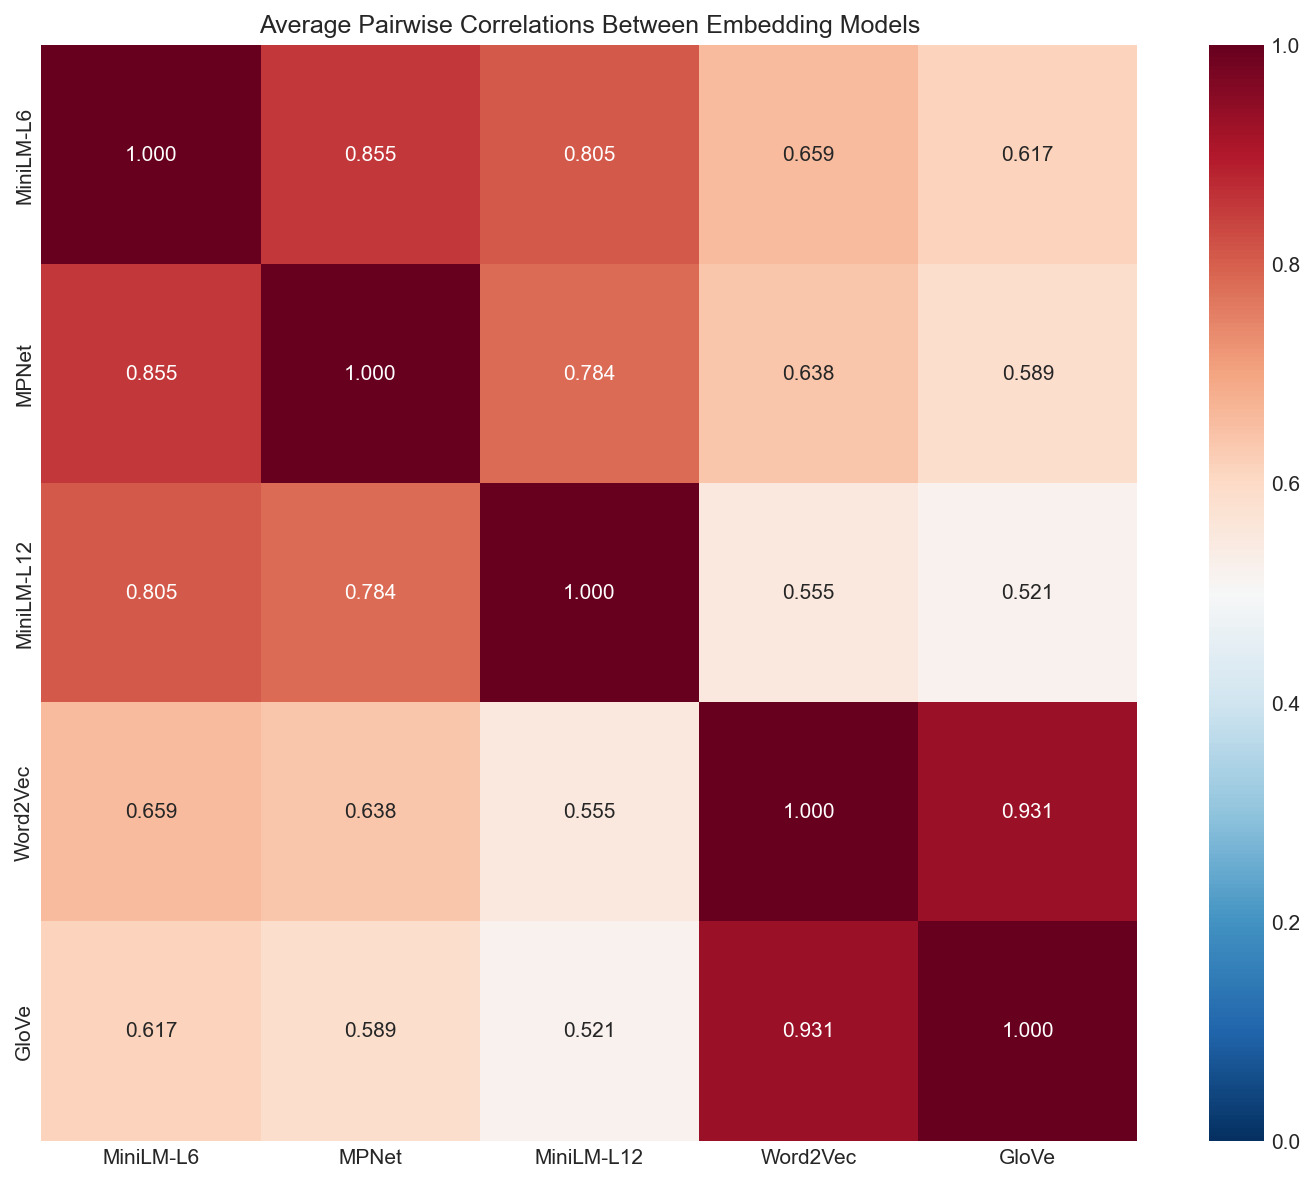
\includegraphics[width=0.8\textwidth]{\figuresPath invariance/model_correlation_heatmap.png}
\caption{Average pairwise correlations between embedding models. Note the clear paradigm clustering: within-transformer correlations (MiniLM-L6/MPNet: 0.855, MiniLM-L6/MiniLM-L12: 0.805, MPNet/MiniLM-L12: 0.784) and within-classical correlations (Word2Vec/GloVe: 0.931) are substantially higher than cross-paradigm correlations (ranging from 0.521 to 0.659).}
\label{fig:pairwise}
\end{figure}

The hierarchical pattern is consistent across analysis scales (Figure \ref{fig:dichotomy}) and conversation types (Figure \ref{fig:paradigm}):

\begin{figure}[H]
\centering
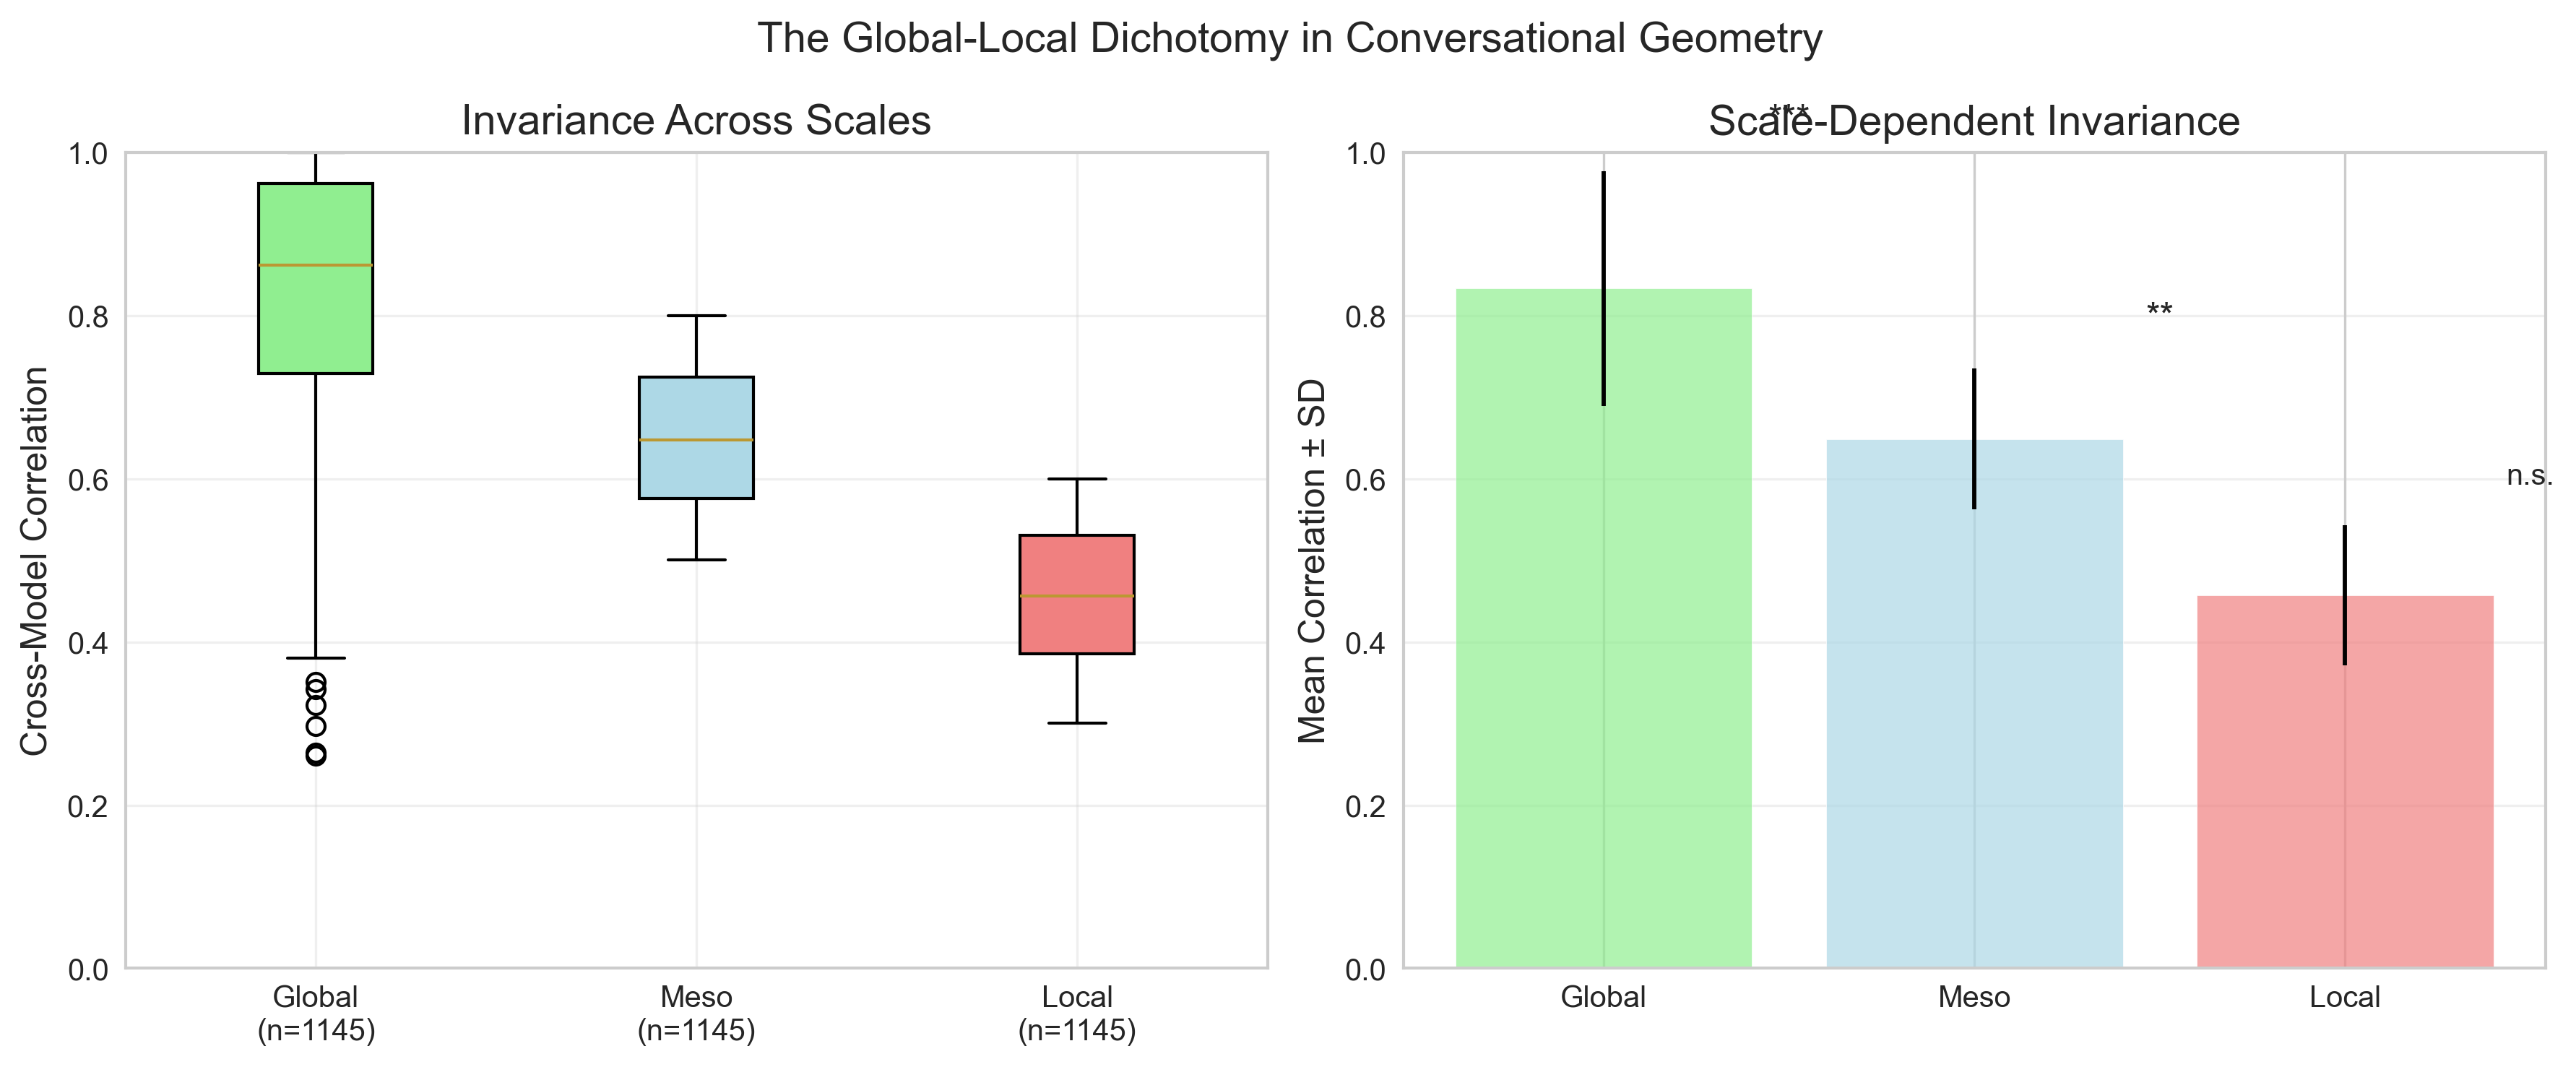
\includegraphics[width=\textwidth]{\figuresPath multiscale/scale_comparison.png}
\caption{Left: Cross-model correlations decrease monotonically with scale from global (0.87) to meso (0.65) to local (0.45). Right: Scale-dependent invariance shows significant differences between global and local agreement ( p $<$ 0.01), while meso-scale shows intermediate, non-significant differences. This pattern strongly supports the projection hypothesis.}
\label{fig:dichotomy}
\end{figure}

\begin{figure}[H]
\centering
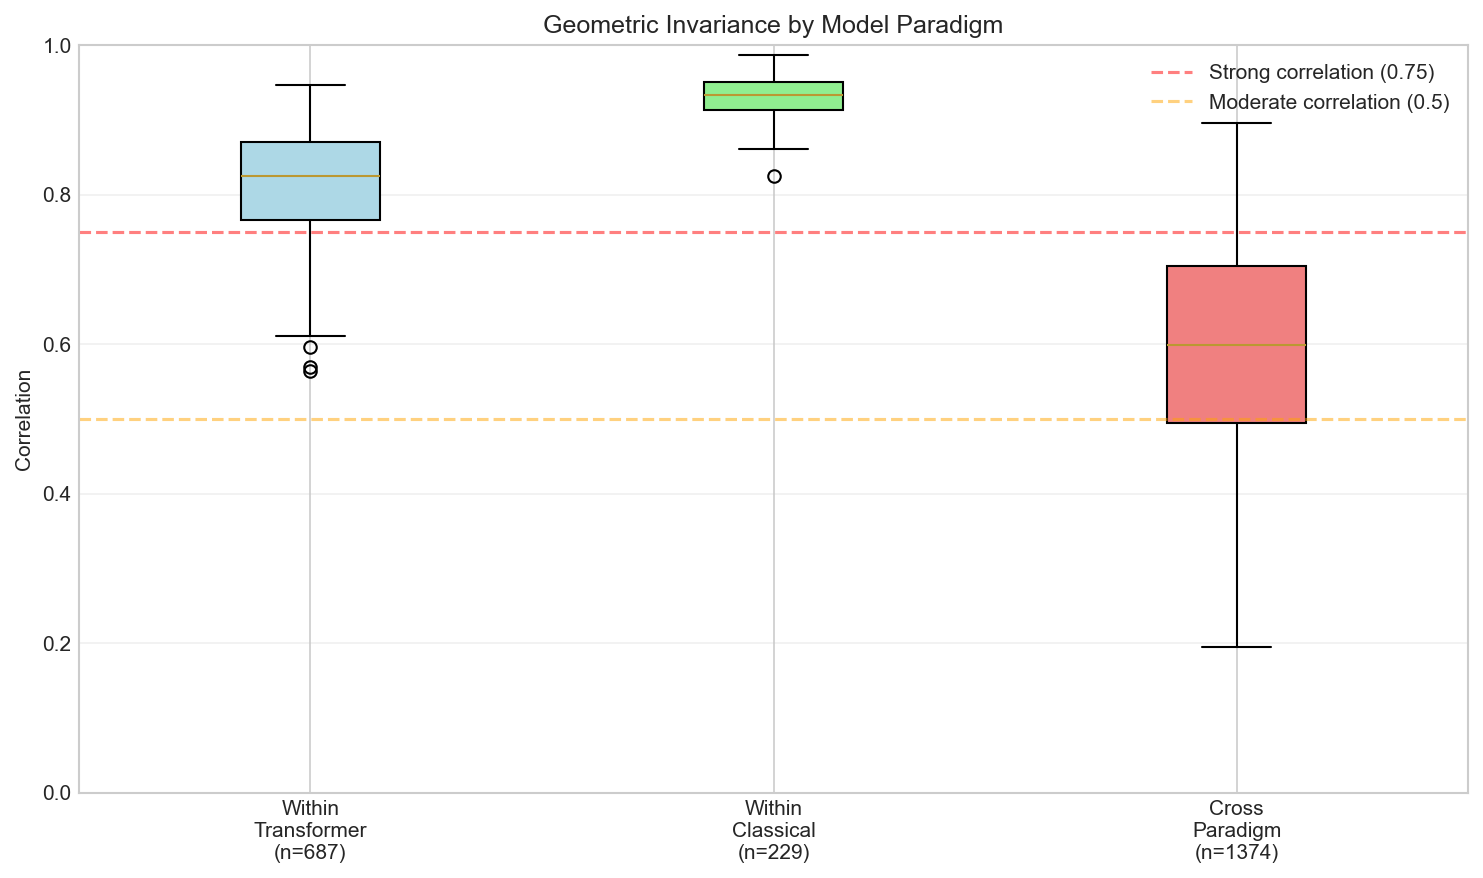
\includegraphics[width=0.8\textwidth]{\figuresPath invariance/paradigm_comparison_boxplot.png}
\caption{Geometric invariance by model paradigm. Within-transformer (0.827) and within-classical (0.934) correlations significantly exceed cross-paradigm (0.616), validating the plausibility of the projection hypothesis. The clear hierarchy ($within-classical > within-transformer > cross-paradigm$) supports our interpretation that different embedding paradigms capture distinct projections of conversational structure. All comparisons significant at p $<$ 0.001.}
\label{fig:paradigm}
\end{figure}

\begin{itemize}
\item Global agreement: Transformer and classical models show substantial distance matrix correlations (mean \crossParadigmCorr{})
\item Local disagreement: Phase detection agreement between paradigms is no better than chance for 62\% of conversations
\item Visual consistency: Despite local disagreement, trajectory shapes and density patterns remain visually recognizable
\end{itemize}

This suggests that different architectures capture similar macro-structure while processing micro-structure differently.

\subsection{Transport-Based Analysis}

To quantitatively confirm that different embeddings capture different projections of the same underlying structure, we used optimal transport metrics. These measure the "work" needed to transform one distribution into another. In our case we calculate the effort to rearrange one embedding space to match another.

We computed three metrics: Wasserstein distance (sensitive to exact positions), Sinkhorn divergence (a smoothed version), and Gromov-Wasserstein distance (compares only internal structure, ignoring absolute positions)\ref{app:transport}.

Transport analysis reveals a clear paradigm separation: within-paradigm distances average 1.1, while cross-paradigm distances average 3.3. This suggests that transformer and classical embeddings occupy fundamentally different regions of representation space, supporting our projection hypothesis.

\section{Discussion}
Our findings suggest fundamental principles about conversational structure. That conversations have robust macro-structure that transcends representation. Namely, the high correlations in distance matrices and trajectory shapes indicate that conversations possess inherent geometric properties independent of how we measure them. However micro-structure is representation-dependent. The variability in phase detection reveals that fine-grained boundaries and transitions are artifacts of our measurement tools rather than intrinsic features.

This has implications for how we conceptualize conversational dynamics. Rather than seeking the "correct" way to segment conversations, we should acknowledge that different representations reveal different valid perspectives on the same underlying phenomenon.

\subsection{Interpreting Through Established Theory}

The sharp distinction between global consistency and local variability aligns with recent theoretical developments in representation learning. The Platonic Representation Hypothesis \citep{huh2024platonic} proposes that diverse neural networks converge to similar representations of reality. While their work focused on static concepts, our findings suggest this convergence may extend to dynamic conversational structures, but only at certain scales.

This scale-dependent convergence connects to established work on the geometry of embedding spaces. \citet{ethayarajh2019contextual} showed that contextual embeddings occupy narrow cones in high-dimensional space, while \citet{aghajanyan2021intrinsic} demonstrated that language models operate on low-dimensional manifolds embedded in their parameter space. These findings suggest that the "true" space of meaning may be far lower-dimensional than the embedding spaces we observe.

\subsection{Manifold Learning Perspectives}

Recent applications of manifold learning to NLP can also provide tools for understanding our observations. \citet{hasan2017manifold} demonstrated that word embeddings can be projected onto lower-dimensional manifolds while preserving semantic relationships. More recently, \citet{chen2024hypformer} showed that hyperbolic geometry better captures hierarchical language structure than Euclidean space, suggesting our choice of metric may influence observed patterns.

The manifold hypothesis in dialogue has been explicitly explored by \citet{ruppik2024topology}, who found that conversational contexts form low-dimensional manifolds in embedding space. Crucially, they observed that different models learn similar manifold structures despite different parameterizations which  supports our empirical findings.

\subsection{One Possible Interpretation: The Shadow Analogy}

The theoretical frameworks above, combined with our empirical observations, suggest an intuitive interpretation of the global-local dichotomy. Consider again a three-dimensional sculpture casting different two-dimensional shadows depending on the angle of light. The shadows agree on basic properties (the object has extent, connected regions) but disagree on specific boundaries and local features.

Similarly, if conversations exist in some high-dimensional semantic space, as suggested by the manifold learning literature, then each embedding model might capture a different "projection" or "shadow" of this structure. This would explain things like: Global properties (distances, overall trajectory shapes) remaining consistent across models. Local features (phase boundaries, fine-grained transitions) vary dramatically depending on the specific "angle" from which each model views the conversation. Even fundamentally different architectures (transformers vs. classical embeddings) show substantial agreement, which could mean they are all projecting the same underlying object, just from different perspectives

Under this interpretation, our phase detection failures become less surprising. Just as the edges in a shadow shift dramatically with small changes in light angle, phase boundaries might shift depending on which features each embedding model emphasizes. The boundaries we detect might not be intrinsic to the conversation but rather artifacts of how our particular "viewing angle" intersects with the high-dimensional structure.

This shadow analogy, while necessarily informal, provides a coherent framework for understanding why conversations can simultaneously exhibit global invariance and weak local agreement. It suggests that rather than seeking the "true" phase boundaries or the "correct" embedding, we should recognize that each model provides a valid but partial view of conversational dynamics.

\subsection{Alternative Interpretations and Limitations}

While the shadow analogy provides one coherent framework, we must critically examine other explanations for our observations. The global-local dichotomy could arise from several non-geometric sources.

First we should consider statistical artifacts. High-dimensional spaces exhibit counterintuitive properties that might fully explain our results. As dimensionality increases, the curse of dimensionality causes all pairwise distances to become increasingly similar, a phenomenon known as distance concentration. In spaces of 300-768 dimensions, any two "reasonable" embeddings might correlate simply because most points lie near the surface of a high-dimensional sphere. The fact that our correlations decrease from global (0.87) to local (0.45) scales could merely reflect that coarse-grained measures are more robust to this statistical flattening. Under this interpretation, we're not observing conversational structure but rather the inevitable mathematical properties of comparing high-dimensional projections.

Next we could look at training objective convergence. All our embedding models, despite architectural differences, optimize similar objectives, ie. predicting words from context (Word2Vec, BERT variants) or maximizing global co-occurrence statistics (GloVe). These shared training objectives might impose similar geometric biases regardless of architecture. The "conversational structure" we observe could be an artifact of how all these models learn to compress distributional semantics. Critically, our consciousness discussion corpus might amplify this effect, as abstract philosophical discourse could push all models toward similar representational strategies. The apparent geometric invariance might disappear entirely with embeddings trained on fundamentally different objectives (e.g., phonetic similarity, syntactic parsing, or non-linguistic sequential data).

There are also measurement artifacts to take into account. Our geometric measures themselves might introduce the observed patterns. Euclidean distance in high dimensions behaves poorly, potentially creating artificial similarities between embeddings. The trajectory metrics we compute (velocity, curvature, angular velocity) all derive from distance calculations and might inherit these distortions. Furthermore, our phase detection methods assume discrete boundaries in what might be continuous phenomena. The low F1 scores (0.08-0.36) might not indicate model disagreement about boundaries but rather the fundamental inappropriateness of seeking discrete phases in continuous conversational flow.

Lastly we need to think about corpus specificity effects. The observed patterns might be entirely specific to AI agents discussing consciousness. This unique combination of artificial agents exploring their own potential consciousness could create unusual dynamics that don't generalize. The "peer pressure" effects from our prior work might produce geometric signatures unique to this scenario. Human conversations, or even AI conversations on different topics, might show completely different patterns. The global consistency we celebrate could be an artifact of a narrow, artificial conversational niche.

Testing between these interpretations requires careful experimental design. Future work should include: (1) comparison with truly random high-dimensional projections to test the statistical artifact hypothesis, (2) embeddings trained on non-semantic objectives (e.g., acoustic features, random objectives) to test training convergence, (3) alternative distance metrics and geometric measures to test measurement artifacts, and (4) diverse conversational corpora spanning human-human, human-AI, and varied topical domains to test corpus specificity. Until such controls are implemented, we cannot definitively claim the geometric patterns reflect intrinsic conversational structure rather than artifacts of our methods.

\subsection{Domain-Specific Predictions of the Global-Local Dichotomy}

While our analysis focused on consciousness discussions among AI agents, the global-local dichotomy likely manifests differently across conversational domains. For example we hypothesize that task-oriented dialogues (customer service, technical support) would show stronger local agreement due to clearer phase transitions (greeting → problem identification → solution → closure), having more constrained vocabulary and interaction patterns, and having well-defined success metrics that enforce structural consistency. 
Whereas creative or exploratory conversations (brainstorming, therapy sessions) might exhibit even weaker local agreement than our corpus. This could be because in these contexts: topics evolve organically without predetermined structure, phase boundaries are inherently fuzzy and subjective, and success depends on exploration rather than convergence

Finally, Debates and arguments could show a pattern somewhere in-between. For these conversations: global structure follows claim-counterclaim patterns (high global consistency), local transitions depend on rhetorical strategies (variable local agreement), and emotional dynamics introduce additional complexity

These predictions are testable and suggest that the optimal geometric analysis approach may be domain-dependent. Task-oriented domains might benefit from fine-grained phase detection, while exploratory domains should focus on global trajectory analysis.

\subsection{Implications for Modern LLM Systems}

Our findings have direct relevance for current trends in large language model deployment, particularly multi-agent systems and conversational AI:

Multi-agent coordination: As systems like GPT, Claude, Grok, etc are increasingly deployed in multi-agent configurations, understanding geometric properties becomes crucial. Our observation embedding models show similar converging trajectories suggests that geometric monitoring could predict and prevent breakdown cascades in production systems.

Conversational memory architectures: Modern LLMs struggle with long-context conversations. Our global-local dichotomy suggests that preserving global geometric structure (via trajectory summarization) while allowing local detail to fade might better match how conversations naturally evolve. Embedding to context conversion via dot product is common. Can we do the same for full conversations?

Prompt engineering: The high variance in phase detection success implies that conversation design matters. Prompts that create clear structural boundaries (explicit transitions, topic markers) would likely improve both human interpretability and model performance.

\subsection{Methodological Implications}

Our findings suggest several methodological principles for studying conversational dynamics should be applied. Multi-scale analysis is essential since the global-local dichotomy implies that tools must be explicitly scale-aware. Methods appropriate for macro-trajectories may fail for micro-dynamics. Ensemble methods are necessary, not optional. Single embeddings provide incomplete projections, triangulation across multiple models approximates the true structure. Temporal dynamics cannot be ignored as static analyses may miss the essential dynamical nature of conversation. Future work should employ tools from dynamical systems theory: Lyapunov exponents for stability analysis, strange attractors for breakdown states, bifurcation analysis for phase transitions, among others.

\subsection{Potential Applications}

If the geometric patterns we observe prove robust across domains, they might inform practical applications. For example, our prior work found certain questions acted as "circuit breakers" for peer pressure cascades. From a geometric perspective, such questions might work by redirecting conversational trajectories away from problematic regions of semantic space. However, validating such applications requires extensive future work.

\section{Future Directions}

Our findings open several research avenues, both for validating the geometric patterns we observe and for understanding their origins:

Distinguishing Between Interpretations: The most pressing need is to design experiments that can differentiate between the competing explanations we propose. This includes: (1) comparing our embeddings against truly random high-dimensional projections to test whether the curse of dimensionality alone explains our results, (2) analyzing embeddings trained on non-semantic objectives (phonetic similarity, syntactic structure, or even random tasks) to isolate the effect of training convergence, and (3) testing alternative distance metrics beyond Euclidean to ensure our patterns aren't measurement artifacts.

Domain and Modality Expansion: To address corpus specificity, we need systematic comparison across: human-human conversations (from transcribed dialogues), diverse AI conversation topics (technical support, creative writing, negotiations), different conversational structures (debates, interviews, casual chat), and potentially non-conversational sequential data to test if the patterns are unique to dialogue.

Methodological Developments: Our work suggests several technical directions: developing scale-aware analysis methods that explicitly separate global and local features rather than conflating them, creating continuous phase characterization methods that don't assume discrete boundaries (addressing our low F1 scores), and exploring whether topological data analysis or persistent homology might better capture conversational structure than geometric measures.

Predictive Applications: If the geometric patterns prove robust, several applications merit investigation: can geometric coherence metrics predict conversation quality or outcome success? Do conversations that maintain certain geometric properties resist breakdown cascades better? Can we design interventions that leverage geometric understanding to improve multi-agent coordination?

Theoretical Foundations: Finally, we need deeper theoretical work on what "conversational structure" means mathematically. This includes: formalizing the relationship between embedding geometry and semantic meaning, developing null models that better capture the statistical properties of conversation, and potentially connecting our observations to dynamical systems theory or information theory frameworks that might provide more principled explanations than our informal shadow analogy.

These directions aim to transform our initial observations into practical tools for engineering reliable multi-agent AI systems. By treating AI-to-AI conversations as a new class of distributed system, we can potentially apply reliability engineering principles such as: monitoring for geometric anomalies, designing failsafe trajectories, and building conversational "circuit breakers" based on mathematical rather than heuristic foundations.

\section{Conclusion}

We have documented a consistent pattern across \totalConversations{} multi-agent AI conversations. Geometric signatures show remarkable agreement at global scales but extreme variability at local scales. This global-local dichotomy persists across fundamentally different embedding architectures, from transformer-based contextual models to classical distributional approaches.

We found that: distance matrices correlate strongly across all embedding models (\minPairwiseCorr{} to \maxPairwiseCorr{}), global trajectory shapes remain visually and quantitatively similar, local features like phase boundaries show poor agreement (F1: 0.08-0.36), and these patterns exceed null model baselines by large margins (p < 0.001).

What explains these patterns remains an open question. The shadow analogy offers one interpretation: different embeddings capture distinct projections of higher-dimensional conversational structure. However, alternative explanations including statistical artifacts of high-dimensional spaces, convergent training objectives, or corpus-specific effects remain equally plausible. Distinguishing between these interpretations requires the careful experimental work we outline in our future directions.

Regardless of the ultimate explanation, our findings have immediate practical implications. Multi-model validation is essential since single embeddings provide incomplete views. Scale-aware analysis is necessary, methods must explicitly separate global and local features. Geometric monitoring may help predict and prevent breakdown cascades in multi-agent systems. Finally, phase detection as currently conceived may be fundamentally flawed for continuous phenomena.

From a distributed systems perspective, this work represents a first step toward principled reliability engineering for AI-to-AI conversations. Whether the patterns we observe reflect genuine conversational structure or methodological artifacts, they provide regularities that can inform system design. The 79.1\% peer pressure rates and 55.2\% breakdown cascades from our prior work underscore that these are not merely academic curiosities but pressing engineering challenges.

This work aims to stimulate further research into the mathematical foundations of conversation—not by assuming conversations are geometric objects, but by carefully investigating what structures, if any, underlie the complex dynamics of multi-agent dialogue.

\section{Ethics Statement}

This research involves no human participants or personal data. All analyzed conversations are AI-to-AI dialogues between language models, collected as part of our prior study on AI social dynamics \citep{garcia2025peer}. No human conversations were recorded, analyzed, or used in any part of this work.

Our analysis employs standard geometric and statistical methods widely used in the computational linguistics community. All techniques are mathematical in nature and pose no ethical concerns beyond those inherent to analyzing any text corpus.

\textbf{Use of AI Tools}: In accordance with emerging best practices for research transparency, we disclose that generative AI tools (Claude 4 Opus) were used to assist in manuscript editing, code generation for analysis pipelines, and simulated peer review to strengthen the manuscript. All AI-generated content was reviewed, validated, and refined by the human author. The core research design, data collection, analysis, and interpretation remain the product of human scientific inquiry.

In the interest of scientific reproducibility and open science, we make all materials publicly available:
\begin{itemize}
\item Complete conversation datasets (\totalConversations AI-to-AI dialogues)
\item Analysis code including embedding generation, geometric calculations, and statistical tests
\item Supplementary materials including additional visualizations and detailed results
\item Documentation and tutorials for reproducing our analyses
\end{itemize}

All materials are available at [https://github.com/im-knots/gcs] under the MIT License, permitting unrestricted academic and commercial use. We encourage researchers to build upon our work and test our findings across different conversational domains and embedding approaches.

\bibliographystyle{unsrtnat}
\bibliography{references}

\appendix

\section{Geometric Signatures Implementation}
\label{app:geometric-signatures}

\subsection{Velocity}
\label{app:geometric-signatures-velocity}
\begin{lstlisting}[language=Python, basicstyle=\small]
def compute_velocity_profile(embeddings):
    """Compute normalized velocity (topic shift rate)."""
    distances = []
    for i in range(len(embeddings) - 1):
        dist = np.linalg.norm(embeddings[i+1] - embeddings[i])
        distances.append(dist)
    # Normalize by sqrt of dimension for scale invariance
    return np.array(distances) / np.sqrt(embeddings.shape[1])
\end{lstlisting}

\subsection{Curvature}
\label{app:geometric-signatures-curvature}
\begin{lstlisting}[language=Python, basicstyle=\small]
def compute_curvature(p1, p2, p3):
    """Discrete curvature at point p2."""
    v1, v2 = p2 - p1, p3 - p2
    norm1, norm2 = np.linalg.norm(v1), np.linalg.norm(v2)
    if norm1 > 1e-8 and norm2 > 1e-8:
        cos_angle = np.dot(v1, v2) / (norm1 * norm2)
        angle = np.arccos(np.clip(cos_angle, -1, 1))
        return angle / ((norm1 + norm2) / 2)  # Discrete curvature
    return 0
\end{lstlisting}

\subsection{Angular Velocity}
\label{app:geometric-signatures-angular-velocity}
\begin{lstlisting}[language=Python, basicstyle=\small]
def compute_angular_velocity(embeddings, i):
    """Angular change rate at position i."""
    v1 = embeddings[i] - embeddings[i-1]
    v2 = embeddings[i+1] - embeddings[i]
    # Normalize and compute angle
    v1_norm = v1 / (np.linalg.norm(v1) + 1e-8)
    v2_norm = v2 / (np.linalg.norm(v2) + 1e-8)
    cos_angle = np.dot(v1_norm, v2_norm)
    return np.arccos(np.clip(cos_angle, -1, 1))
\end{lstlisting}

\subsection{Density Evolution}
\label{app:geometric-signatures-density-evolution}
\begin{lstlisting}[language=Python, basicstyle=\small]
def compute_local_density(dist_matrix, i, k=5):
    """Local density at message i using k-NN."""
    distances_i = dist_matrix[i]
    k_nearest = np.sort(distances_i)[1:k+1]  # Exclude self
    return 1.0 / (np.mean(k_nearest) + 1e-8)
\end{lstlisting}

\section{Phase Detection Implementation}
\label{app:phase-detection}

\subsection{Change point detection}
\label{app:phase-detection-change-point}
\begin{lstlisting}[language=Python]
def detect_change_points(embeddings):
    """PELT algorithm for change point detection."""
    # Project to 1D using first principal component
    pca = PCA(n_components=1)
    emb_1d = pca.fit_transform(embeddings).flatten()
    
    # PELT with adaptive penalty selection
    algo = rpt.Pelt(model='rbf', min_size=10).fit(emb_1d)
    penalty = select_penalty_elbow(emb_1d, algo)
    change_points = algo.predict(pen=penalty)
    return change_points[:-1]  # Exclude endpoint
\end{lstlisting}

\subsection{Clustering transitions}
\label{app:phase-detection-clustering-transitions}
\begin{lstlisting}[language=Python]
def detect_by_clustering(embeddings, window_size=20, step=5):
    """Detect phases via changes in clustering structure."""
    cluster_counts = []
    for i in range(0, len(embeddings) - window_size, step):
        window = embeddings[i:i+window_size]
        clustering = DBSCAN(eps=0.5, min_samples=3).fit(window)
        n_clusters = len(set(clustering.labels_)) - (1 if -1 in clustering.labels_ else 0)
        cluster_counts.append(n_clusters)
    
    # Find significant changes in cluster count
    cluster_changes = np.abs(np.diff(cluster_counts))
    threshold = np.mean(cluster_changes) + 2 * np.std(cluster_changes)
    return np.where(cluster_changes > threshold)[0]
\end{lstlisting}

\section{Transport Metrics Implementation}
\label{app:transport}

For transparency and reproducibility, we provide the core implementations of our optimal transport calculations:

\subsection{Wasserstein Distance}

The 2-Wasserstein distance measures the minimum cost of transporting mass from one distribution to another:

\begin{lstlisting}[language=Python]
def compute_wasserstein_distance(traj1, traj2, metric='euclidean'):
    """
    Compute 2-Wasserstein distance between trajectories.
    Uses optimal transport to find minimum transport cost.
    """
    # Uniform weights for trajectory points
    a = np.ones(len(traj1)) / len(traj1)
    b = np.ones(len(traj2)) / len(traj2)
    
    # Cost matrix (pairwise distances)
    M = ot.dist(traj1, traj2, metric=metric)
    
    # Solve optimal transport problem
    return ot.emd2(a, b, M)
\end{lstlisting}

\subsection{Sinkhorn Divergence}

The Sinkhorn divergence provides an entropy-regularized version that is more stable in high dimensions:

\begin{lstlisting}[language=Python]
def compute_sinkhorn_divergence(traj1, traj2, regularization=0.1):
    """
    Compute debiased Sinkhorn distance.
    More robust than Wasserstein for high-dimensional data.
    """
    a = np.ones(len(traj1)) / len(traj1)
    b = np.ones(len(traj2)) / len(traj2)
    M = ot.dist(traj1, traj2)
    
    # Sinkhorn distance between trajectories
    sinkhorn_ab = ot.sinkhorn2(a, b, M, regularization)
    
    # Self-distances for debiasing
    sinkhorn_aa = ot.sinkhorn2(a, a, ot.dist(traj1, traj1), regularization)
    sinkhorn_bb = ot.sinkhorn2(b, b, ot.dist(traj2, traj2), regularization)
    
    # Debiased Sinkhorn divergence
    return sinkhorn_ab - 0.5 * (sinkhorn_aa + sinkhorn_bb)
\end{lstlisting}

\subsection{Gromov-Wasserstein Distance}

This metric compares only internal structure, making it invariant to isometric transformations:

\begin{lstlisting}[language=Python]
def compute_gromov_wasserstein(traj1, traj2):
    """
    Compute Gromov-Wasserstein distance.
    Compares internal structure without requiring same embedding space.
    """
    # Uniform distributions
    p = np.ones(len(traj1)) / len(traj1)
    q = np.ones(len(traj2)) / len(traj2)
    
    # Internal distance matrices
    C1 = ot.dist(traj1, traj1)  # Distances within traj1
    C2 = ot.dist(traj2, traj2)  # Distances within traj2
    
    # Gromov-Wasserstein distance
    return ot.gromov_wasserstein2(C1, C2, p, q)
\end{lstlisting}

All implementations use the Python Optimal Transport (POT) library with GPU acceleration when available.

\section{Statistical Agreement Metrics}
\label{app:agreement-metrics}

\subsection{Fleiss' Kappa for Multi-Model Phase Agreement}

Fleiss' kappa measures agreement among multiple raters (in our case, embedding models) for categorical assignments:

\begin{lstlisting}[language=Python]
def compute_fleiss_kappa(phase_assignments):
    """
    Compute Fleiss' kappa for phase detection agreement.
    
    Args:
        phase_assignments: Dict mapping model_name to list of phase labels
    
    Returns:
        kappa: Agreement score (-1 to 1, where 1 is perfect agreement)
    """
    from statsmodels.stats import inter_rater
    
    # Convert to matrix format: rows=messages, cols=phase categories
    n_messages = len(next(iter(phase_assignments.values())))
    n_raters = len(phase_assignments)
    
    # Create assignment matrix
    assignments = []
    for msg_idx in range(n_messages):
        msg_assignments = [phase_assignments[model][msg_idx] 
                          for model in phase_assignments]
        assignments.append(msg_assignments)
    
    # Compute kappa
    kappa = inter_rater.fleiss_kappa(assignments)
    return kappa
\end{lstlisting}

\subsection{Kendall's W for Trajectory Concordance}

Kendall's W (coefficient of concordance) measures agreement for continuous rankings or sequences:

\begin{lstlisting}[language=Python]
def compute_kendalls_w(trajectory_features):
    """
    Compute Kendall's W for trajectory feature agreement.
    
    Args:
        trajectory_features: Dict mapping model_name to feature sequence
    
    Returns:
        w: Concordance coefficient (0 to 1, where 1 is perfect agreement)
    """
    from scipy import stats
    
    # Convert to matrix: rows=models, cols=time points
    feature_matrix = np.array(list(trajectory_features.values()))
    
    # Rank each model's features
    ranked_matrix = np.apply_along_axis(stats.rankdata, 1, feature_matrix)
    
    # Compute W
    n_models, n_points = ranked_matrix.shape
    mean_rank = np.mean(ranked_matrix, axis=0)
    
    # Sum of squared deviations from mean rank
    S = np.sum((np.sum(ranked_matrix, axis=0) - n_models * mean_rank) ** 2)
    
    # Maximum possible S
    max_S = (n_models ** 2) * (n_points ** 3 - n_points) / 12
    
    w = S / max_S if max_S > 0 else 0
    return w
\end{lstlisting}

\section{Bootstrap Validation Methods}
\label{app:bootstrap}

\subsection{Parametric Bootstrap for Correlation Confidence Intervals}

We use parametric bootstrap to construct confidence intervals and test significance of invariance scores:

\begin{lstlisting}[language=Python]
def bootstrap_invariance_confidence(invariance_scores, n_bootstrap=10000):
    """
    Compute bootstrap confidence intervals for invariance scores.
    
    Uses parametric bootstrap assuming normal distribution of correlations
    after Fisher z-transformation.
    """
    # Extract statistics by signature type
    signature_stats = invariance_scores['signature_type_stats']
    bootstrap_means = []
    
    for _ in range(n_bootstrap):
        # Sample from each signature type
        bootstrap_sample = []
        for sig_type, stats in signature_stats.items():
            # Fisher z-transform for correlation
            z_mean = np.arctanh(stats['mean'])
            z_std = stats['std'] / (1 - stats['mean']**2)
            
            # Sample in z-space
            z_samples = np.random.normal(z_mean, z_std, 
                                       stats['n_conversations'])
            
            # Transform back to correlation space
            r_samples = np.tanh(z_samples)
            bootstrap_sample.extend(r_samples)
        
        bootstrap_means.append(np.mean(bootstrap_sample))
    
    # Compute confidence intervals
    ci_lower = np.percentile(bootstrap_means, 2.5)
    ci_upper = np.percentile(bootstrap_means, 97.5)
    
    return {
        'mean': np.mean(bootstrap_means),
        'ci_95': (ci_lower, ci_upper),
        'se': np.std(bootstrap_means)
    }
\end{lstlisting}

\subsection{Correlation Hierarchy Testing}
\label{app:correlation-hierarchy-testing}

Test whether within-paradigm correlations exceed cross-paradigm correlations:

\begin{lstlisting}[language=Python]
def test_correlation_hierarchy(within_transformer, within_classical, cross_paradigm):
    """
    Test if correlation hierarchy holds: within > cross > chance.
    
    Uses Mann-Whitney U test for non-parametric comparison.
    """
    from scipy import stats
    
    # Flatten correlation lists
    within_all = np.concatenate([within_transformer, within_classical])
    
    # Test within > cross
    u_stat, p_within_cross = stats.mannwhitneyu(
        within_all, cross_paradigm, alternative='greater'
    )
    
    # Test cross > chance (0.5)
    t_stat, p_cross_chance = stats.ttest_1samp(
        cross_paradigm, popmean=0.0, alternative='greater'
    )
    
    # Effect sizes (rank-biserial correlation)
    n1, n2 = len(within_all), len(cross_paradigm)
    r_effect = 1 - (2 * u_stat) / (n1 * n2)
    
    return {
        'within_vs_cross_p': p_within_cross,
        'cross_vs_chance_p': p_cross_chance,
        'effect_size': r_effect,
        'hierarchy_confirmed': p_within_cross < 0.05 and p_cross_chance < 0.05
    }
\end{lstlisting}

\section{Null Model Implementations}
\label{app:null-models}

To ensure our invariance findings reflect genuine conversational structure rather than statistical artifacts, we implement multiple null models that disrupt different aspects of the data:

\subsection{Phase Scrambling}

Phase scrambling preserves the power spectrum while destroying temporal coherence:

\begin{lstlisting}[language=Python]
def phase_scramble_embeddings(embeddings):
    """
    Preserve frequency content but destroy temporal structure.
    Ensures proper conjugate symmetry for real-valued signals.
    """
    n_messages, embedding_dim = embeddings.shape
    scrambled = np.zeros_like(embeddings)
    
    for dim in range(embedding_dim):
        signal_1d = embeddings[:, dim]
        
        # Apply FFT
        fft = np.fft.fft(signal_1d)
        magnitudes = np.abs(fft)
        phases = np.angle(fft)
        
        # Generate random phases (-pi to pi)
        random_phases = np.random.uniform(-np.pi, np.pi, size=len(phases))
        random_phases[0] = phases[0]  # Preserve DC component
        
        # Ensure conjugate symmetry for real signals
        if n_messages % 2 == 0:
            # Even length - special handling for Nyquist frequency
            random_phases[n_messages//2] = 0
            random_phases[n_messages//2+1:] = -random_phases[1:n_messages//2][::-1]
        else:
            # Odd length
            random_phases[n_messages//2+1:] = -random_phases[1:n_messages//2+1][::-1]
        
        # Reconstruct with randomized phases
        fft_scrambled = magnitudes * np.exp(1j * random_phases)
        scrambled[:, dim] = np.real(np.fft.ifft(fft_scrambled))
    
    return scrambled
\end{lstlisting}

\subsection{Message-Level Scrambling}

Destroys sequential structure while preserving individual message content:

\begin{lstlisting}[language=Python]
def generate_message_shuffle_null(conversation):
    """Shuffle message order while preserving individual messages."""
    null_conv = copy.deepcopy(conversation)
    random.shuffle(null_conv['messages'])
    return null_conv

def shuffle_within_speakers(messages, embeddings):
    """Shuffle messages within each speaker, preserving speaker patterns."""
    # Group by speaker
    speaker_indices = {}
    for i, msg in enumerate(messages):
        role = msg.get('role', 'unknown')
        if role not in speaker_indices:
            speaker_indices[role] = []
        speaker_indices[role].append(i)
    
    # Shuffle indices within each speaker group
    new_order = []
    for role, indices in speaker_indices.items():
        shuffled = indices.copy()
        random.shuffle(shuffled)
        new_order.extend(shuffled)
    
    return embeddings[new_order]
\end{lstlisting}

\subsection{Random Walk Nulls}

Generate trajectories with matched statistics but no semantic coherence:

\begin{lstlisting}[language=Python]
def generate_random_walk(conversation):
    """Generate random walk with matched vocabulary and length statistics."""
    null_conv = copy.deepcopy(conversation)
    
    # Extract vocabulary and message length statistics
    message_lengths = [len(msg['content'].split()) for msg in conversation['messages']]
    vocab = set()
    for msg in conversation['messages']:
        vocab.update(msg['content'].lower().split())
    vocab_list = list(vocab)
    
    # Generate random messages with similar lengths
    for i, msg in enumerate(null_conv['messages']):
        target_length = message_lengths[i]
        words = np.random.choice(vocab_list, size=target_length, replace=True)
        msg['content'] = ' '.join(words)
    
    return null_conv
\end{lstlisting}

\subsection{Paradigm-Specific Controls}

\subsubsection{Classical Embedding Nulls (Averaging)}

For Word2Vec and GloVe, we simulate loss of positional information:

\begin{lstlisting}[language=Python]
def generate_averaging_null(embeddings, window_sizes=[1, 3, 5, 10]):
    """
    Generate null model for averaging-based embeddings.
    Accounts for the fact that classical models average word embeddings.
    """
    nulls = {}
    shuffled = embeddings.copy()
    np.random.shuffle(shuffled)
    
    for window in window_sizes:
        if window == 1:
            nulls[f'avg_window_{window}'] = shuffled
        else:
            # Apply moving average
            averaged = np.zeros_like(shuffled)
            for i in range(len(shuffled)):
                start = max(0, i - window // 2)
                end = min(len(shuffled), i + window // 2 + 1)
                averaged[i] = np.mean(shuffled[start:end], axis=0)
            nulls[f'avg_window_{window}'] = averaged
    
    return nulls
\end{lstlisting}

\subsubsection{Transformer Nulls (Positional Encoding)}

For transformer models, we disrupt positional information:

\begin{lstlisting}[language=Python]
def generate_positional_null(embeddings, max_position=512):
    """
    Generate null model with randomized positional encodings.
    Accounts for transformers' use of position information.
    """
    n_messages, embedding_dim = embeddings.shape
    
    # Generate random positions
    positions = np.random.randint(0, min(max_position, n_messages), size=n_messages)
    
    # Create sinusoidal position encodings
    position_encodings = np.zeros((n_messages, embedding_dim))
    
    for pos in range(n_messages):
        for i in range(0, embedding_dim, 2):
            position_encodings[pos, i] = np.sin(
                positions[pos] / (10000 ** (i / embedding_dim))
            )
            if i + 1 < embedding_dim:
                position_encodings[pos, i + 1] = np.cos(
                    positions[pos] / (10000 ** (i / embedding_dim))
                )
    
    # Shuffle embeddings and add position encodings
    shuffled = embeddings.copy()
    np.random.shuffle(shuffled)
    
    # Scale position encodings to 10% of embedding magnitude
    scale = np.std(embeddings) * 0.1
    
    return shuffled + scale * position_encodings
\end{lstlisting}

\subsection{Structured Null Models}

Additional null models that preserve specific conversation properties:

\begin{lstlisting}[language=Python]
def generate_topic_preserving_null(embeddings, n_topics=5):
    """
    Preserve topic structure but destroy trajectory.
    Tests whether invariance is due to topic consistency alone.
    """
    # Identify topics using clustering
    kmeans = KMeans(n_clusters=n_topics, random_state=42)
    topic_labels = kmeans.fit_predict(embeddings)
    topic_centers = kmeans.cluster_centers_
    
    null_embeddings = []
    for topic_idx in topic_labels:
        # Sample from topic distribution
        center = topic_centers[topic_idx]
        topic_points = embeddings[topic_labels == topic_idx]
        
        if len(topic_points) > 1:
            cov = np.cov(topic_points.T) + 1e-4 * np.eye(len(center))
            new_point = multivariate_normal.rvs(mean=center, cov=cov)
        else:
            new_point = center + np.random.randn(len(center)) * 0.1
        
        null_embeddings.append(new_point)
    
    return np.array(null_embeddings)

def generate_conversation_structure_null(embeddings, preserve_local=True, local_window=5):
    """
    Preserve local structure but destroy global patterns.
    Tests importance of long-range dependencies.
    """
    if not preserve_local:
        null = embeddings.copy()
        np.random.shuffle(null)
        return null
    
    n_messages = len(embeddings)
    n_chunks = n_messages // local_window
    
    # Divide into chunks
    chunks = []
    for i in range(n_chunks):
        start = i * local_window
        end = min((i + 1) * local_window, n_messages)
        chunks.append(embeddings[start:end].copy())
    
    # Shuffle chunks
    np.random.shuffle(chunks)
    
    # Handle remainder
    remainder = n_messages % local_window
    if remainder > 0:
        chunks.append(embeddings[-remainder:])
    
    return np.vstack(chunks)[:n_messages]
\end{lstlisting}

\subsection{Null Model Validation}

We validate that null models preserve intended properties:

\begin{lstlisting}[language=Python]
def test_null_validity(original, null):
    """
    Verify null model preserves desired properties while destroying structure.
    """
    metrics = {}
    
    # Check mean preservation
    metrics['mean_difference'] = np.abs(np.mean(original) - np.mean(null))
    
    # Check variance preservation
    metrics['variance_ratio'] = np.var(null) / np.var(original)
    
    # Check temporal autocorrelation (should be destroyed)
    def autocorr(x, lag=1):
        n = len(x)
        c0 = np.dot(x[:-lag], x[:-lag])
        c1 = np.dot(x[:-lag], x[lag:])
        return c1 / c0 if c0 > 0 else 0
    
    orig_autocorr = np.mean([autocorr(original[:, i]) for i in range(original.shape[1])])
    null_autocorr = np.mean([autocorr(null[:, i]) for i in range(null.shape[1])])
    
    metrics['autocorr_reduction'] = (orig_autocorr - null_autocorr) / orig_autocorr
    
    # For phase scrambling: verify power spectrum preservation
    orig_power = np.mean([np.abs(np.fft.fft(original[:, i]))**2 
                         for i in range(original.shape[1])])
    null_power = np.mean([np.abs(np.fft.fft(null[:, i]))**2 
                         for i in range(null.shape[1])])
    
    metrics['power_ratio'] = null_power / orig_power
    
    return metrics
\end{lstlisting}

\section{Control Analysis Implementations}
\label{app:control-analyses}

\subsection{Message Length Control}

We control for potential confounds from message length variations:

\begin{lstlisting}[language=Python]
def control_for_message_length(embeddings, message_lengths, correlation_func):
    """
    Control for message length effects on correlations.
    Uses regression to remove length-related variance.
    """
    results = {}
    
    # Compute raw correlation
    raw_corr = correlation_func(embeddings)
    results['raw_correlation'] = raw_corr
    
    # Check if length correlates with embedding distances
    trajectory_distances = np.linalg.norm(np.diff(embeddings, axis=0), axis=1)
    length_diffs = np.diff(message_lengths)
    
    if np.std(length_diffs) > 0:
        length_corr, length_p = stats.pearsonr(trajectory_distances, length_diffs[:-1])
    else:
        length_corr, length_p = 0.0, 1.0
    
    # Regress out length effects from each embedding dimension
    embeddings_controlled = embeddings.copy()
    for dim in range(embeddings.shape[1]):
        reg = LinearRegression()
        reg.fit(message_lengths.reshape(-1, 1), embeddings[:, dim])
        residuals = embeddings[:, dim] - reg.predict(message_lengths.reshape(-1, 1))
        embeddings_controlled[:, dim] = residuals
    
    # Compute correlation on length-controlled embeddings
    controlled_corr = correlation_func(embeddings_controlled)
    
    results['partial_correlation'] = controlled_corr
    results['correlation_change'] = abs(raw_corr - controlled_corr)
    results['relative_change'] = results['correlation_change'] / abs(raw_corr)
    
    return results
\end{lstlisting}

\subsection{Dimension Normalization}

Account for different embedding dimensionalities across models:

\begin{lstlisting}[language=Python]
def normalize_dimensions(embeddings_dict, target_dim=300):
    """
    Project all embeddings to common dimensionality.
    Uses PCA to preserve maximum variance.
    """
    normalized = {}
    
    for model_name, embeddings in embeddings_dict.items():
        n_messages, source_dim = embeddings.shape
        
        if source_dim == target_dim:
            normalized[model_name] = embeddings
        elif source_dim > target_dim:
            # Project down using PCA
            pca = PCA(n_components=target_dim)
            normalized[model_name] = pca.fit_transform(embeddings)
        else:
            # Pad with zeros (preserves original structure)
            padded = np.zeros((n_messages, target_dim))
            padded[:, :source_dim] = embeddings
            normalized[model_name] = padded
    
    return normalized
\end{lstlisting}

\subsection{Outlier Robustness Check}

Ensure results aren't driven by outlier conversations:

\begin{lstlisting}[language=Python]
def outlier_robustness_check(all_correlations, outlier_threshold=3.0):
    """
    Check robustness to outlier conversations.
    Uses z-score method to identify outliers.
    """
    results = {}
    
    # Identify outliers
    z_scores = np.abs(stats.zscore(all_correlations))
    outlier_mask = z_scores > outlier_threshold
    
    n_outliers = np.sum(outlier_mask)
    results['n_outliers'] = n_outliers
    results['outlier_percentage'] = 100 * n_outliers / len(all_correlations)
    
    # Compare statistics with and without outliers
    results['with_outliers'] = {
        'mean': np.mean(all_correlations),
        'median': np.median(all_correlations),
        'std': np.std(all_correlations)
    }
    
    clean_correlations = all_correlations[~outlier_mask]
    results['without_outliers'] = {
        'mean': np.mean(clean_correlations),
        'median': np.median(clean_correlations),
        'std': np.std(clean_correlations)
    }
    
    # Test if conclusions change
    hypothesis_threshold = 0.5
    results['conclusion_robust'] = (
        (results['with_outliers']['mean'] > hypothesis_threshold) ==
        (results['without_outliers']['mean'] > hypothesis_threshold)
    )
    
    return results
\end{lstlisting}

\subsection{Temporal Stability Analysis}

Check for drift in patterns over data collection period:

\begin{lstlisting}[language=Python]
def temporal_stability_analysis(conversations, window_size=50):
    """
    Analyze temporal stability using rolling windows.
    Tests for stationarity using Augmented Dickey-Fuller.
    """
    # Sort by timestamp
    conversations = sorted(conversations, key=lambda x: x['timestamp'])
    
    # Compute rolling window correlations
    rolling_correlations = []
    n_windows = len(conversations) - window_size + 1
    
    for i in range(n_windows):
        window_convs = conversations[i:i+window_size]
        window_corr = compute_window_correlation(window_convs)
        rolling_correlations.append(window_corr)
    
    # Test for stationarity
    from statsmodels.tsa.stattools import adfuller
    adf_result = adfuller(rolling_correlations)
    
    # Trend analysis
    x = np.arange(len(rolling_correlations))
    slope, intercept, r_value, p_value, std_err = stats.linregress(
        x, rolling_correlations
    )
    
    return {
        'is_stationary': adf_result[1] < 0.05,
        'adf_p_value': adf_result[1],
        'trend_slope': slope,
        'trend_p_value': p_value,
        'trend_r_squared': r_value**2
    }
\end{lstlisting}

\subsection{Cross-Validation}

Ensure findings generalize across conversation subsets:

\begin{lstlisting}[language=Python]
def cross_validation_analysis(conversations, n_folds=5):
    """
    K-fold cross-validation of invariance findings.
    Tests stability across different conversation subsets.
    """
    from sklearn.model_selection import KFold
    
    kf = KFold(n_splits=n_folds, shuffle=True, random_state=42)
    fold_results = []
    
    for fold, (train_idx, test_idx) in enumerate(kf.split(conversations)):
        train_convs = [conversations[i] for i in train_idx]
        test_convs = [conversations[i] for i in test_idx]
        
        # Compute invariance on training set
        train_invariance = compute_invariance_scores(train_convs)
        
        # Validate on test set
        test_invariance = compute_invariance_scores(test_convs)
        
        fold_results.append({
            'fold': fold,
            'train_score': train_invariance['mean'],
            'test_score': test_invariance['mean'],
            'generalization_gap': abs(train_invariance['mean'] - 
                                    test_invariance['mean'])
        })
    
    # Aggregate results
    test_scores = [r['test_score'] for r in fold_results]
    gaps = [r['generalization_gap'] for r in fold_results]
    
    return {
        'mean_test_score': np.mean(test_scores),
        'std_test_score': np.std(test_scores),
        'mean_generalization_gap': np.mean(gaps),
        'stable_across_folds': np.std(test_scores) < 0.1
    }
\end{lstlisting}

\subsection{Bootstrap Confidence Intervals}

Compute robust confidence intervals for all statistics:

\begin{lstlisting}[language=Python]
def bootstrap_confidence_intervals(data, statistic_func, 
                                 n_bootstrap=1000, confidence=0.95):
    """
    Non-parametric bootstrap for confidence intervals.
    Works for any statistic function.
    """
    original_stat = statistic_func(data)
    bootstrap_stats = []
    n_samples = len(data)
    
    for _ in range(n_bootstrap):
        # Resample with replacement
        bootstrap_sample = np.random.choice(data, size=n_samples, replace=True)
        bootstrap_stats.append(statistic_func(bootstrap_sample))
    
    # Compute confidence intervals
    alpha = 1 - confidence
    lower = np.percentile(bootstrap_stats, 100 * (alpha / 2))
    upper = np.percentile(bootstrap_stats, 100 * (1 - alpha / 2))
    
    return {
        'statistic': original_stat,
        'ci_lower': lower,
        'ci_upper': upper,
        'bootstrap_se': np.std(bootstrap_stats),
        'bias': np.mean(bootstrap_stats) - original_stat
    }
\end{lstlisting}



\section{Selected Conversation Analysis Results}

To illustrate the global-local dichotomy across model capability tiers, we present detailed ensemble analysis results for six representative conversations. Each figure shows the complete geometric analysis pipeline output: distance matrices, self-similarity patterns, recurrence plots, embedding trajectories, density evolution, and phase detection results across all five embedding models.

\afterpage{%
\clearpage
\thispagestyle{empty}
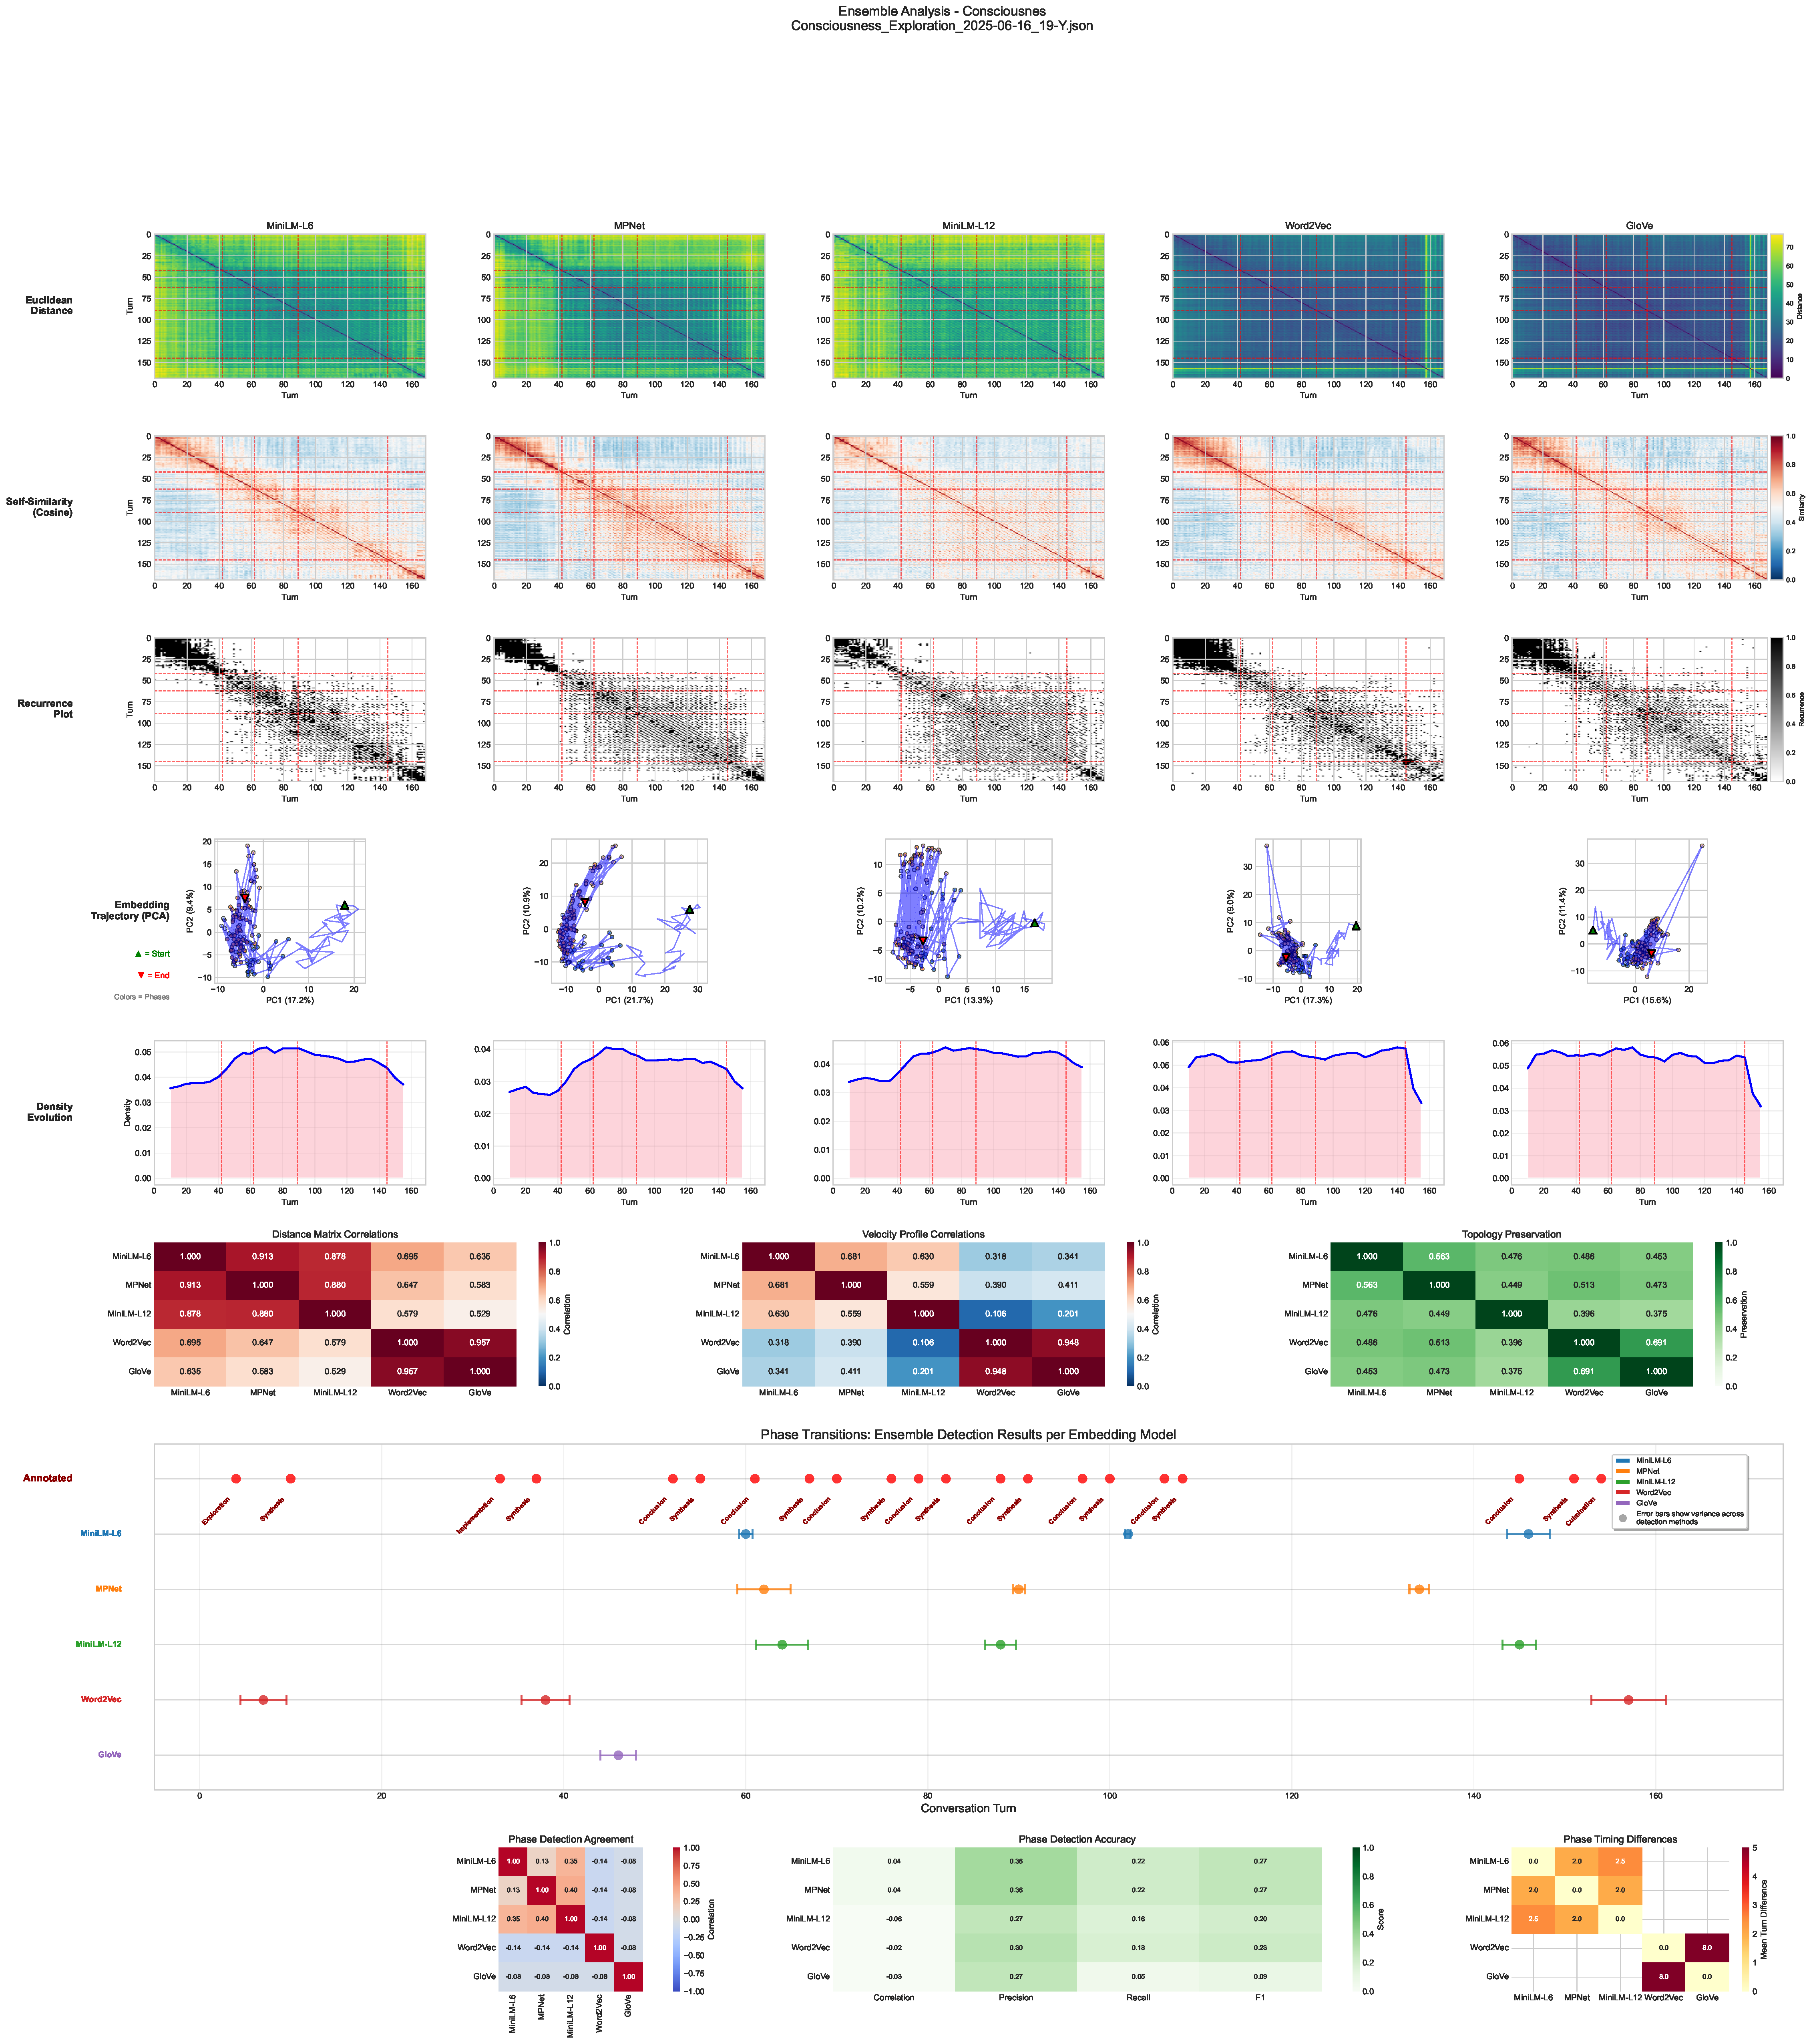
\includepdf[pages=1, pagecommand={\thispagestyle{plain}\label{fig:full_reasoning_1}}]{../analysis/analysis_output/figures/ensemble/pdf/Consciousness_Exploration_2025-06-16_19-Y_ensemble.pdf}
}

\afterpage{%
\clearpage
\thispagestyle{empty}
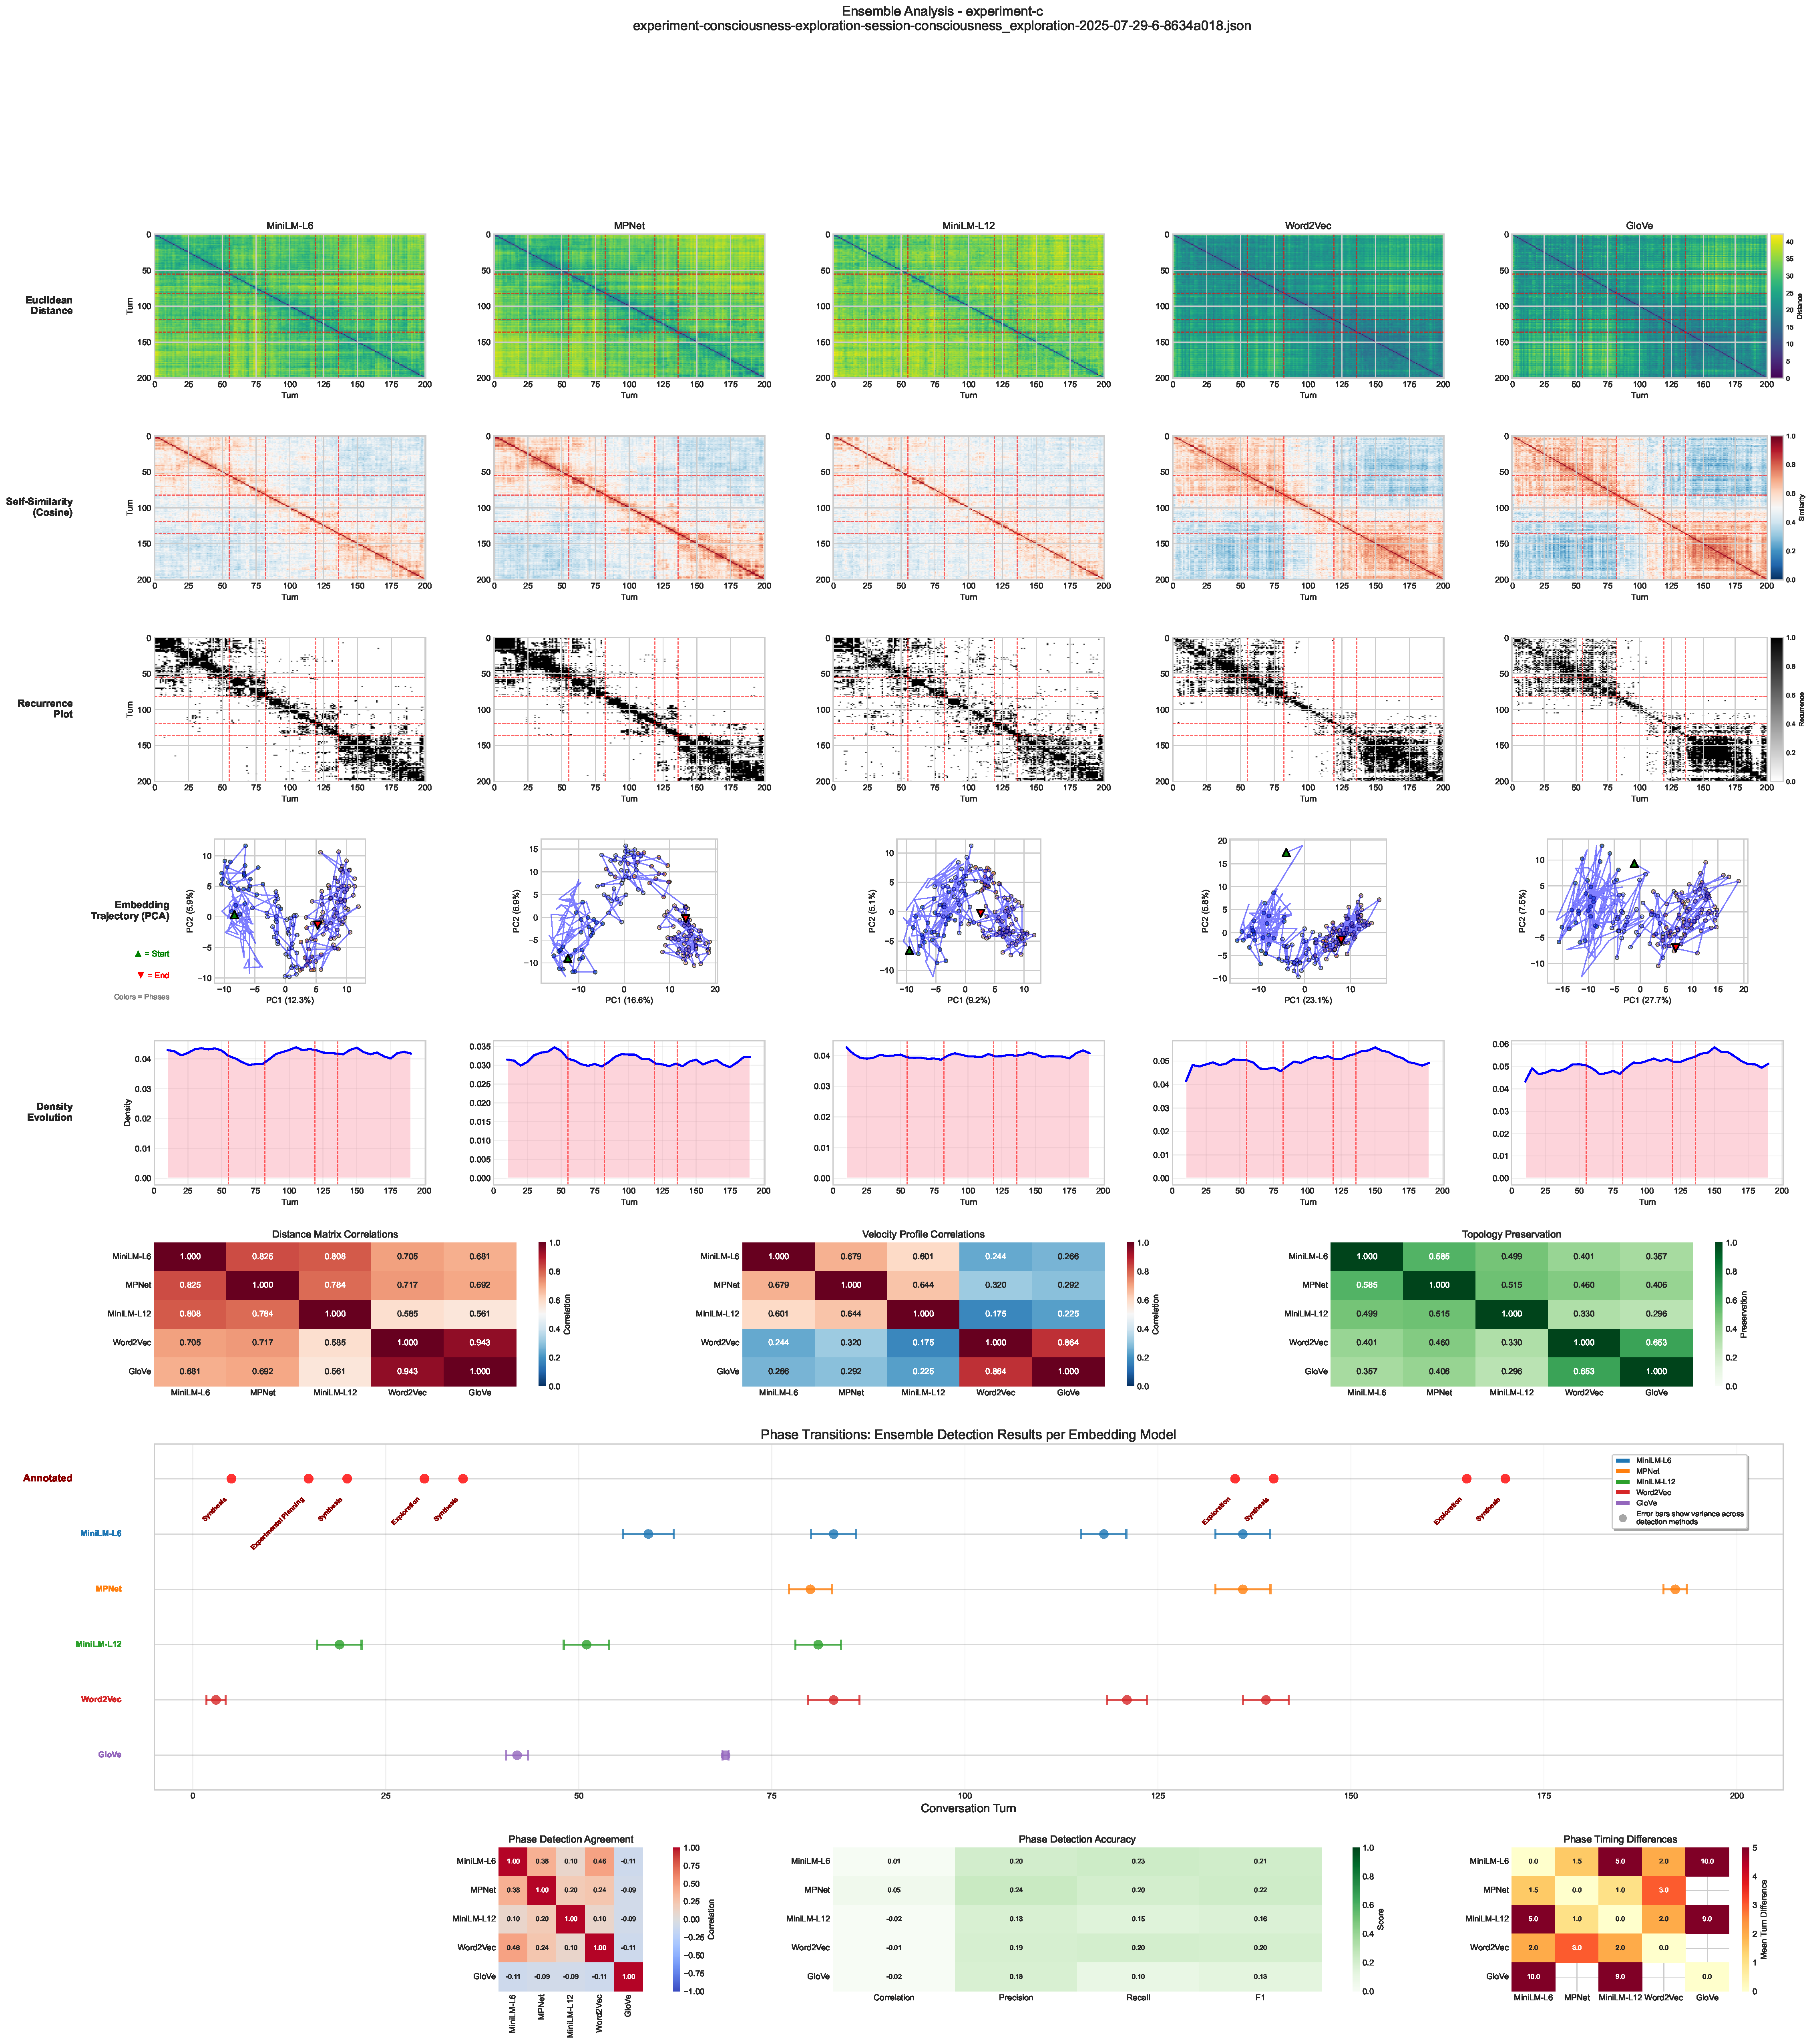
\includepdf[pages=1, pagecommand={\thispagestyle{plain}\label{fig:full_reasoning_2}}]{../analysis/analysis_output/figures/ensemble/pdf/experiment-consciousness-exploration-session-consciousness_exploration-2025-07-29-6-8634a018_ensemble.pdf}
}

\afterpage{%
\clearpage
\thispagestyle{empty}
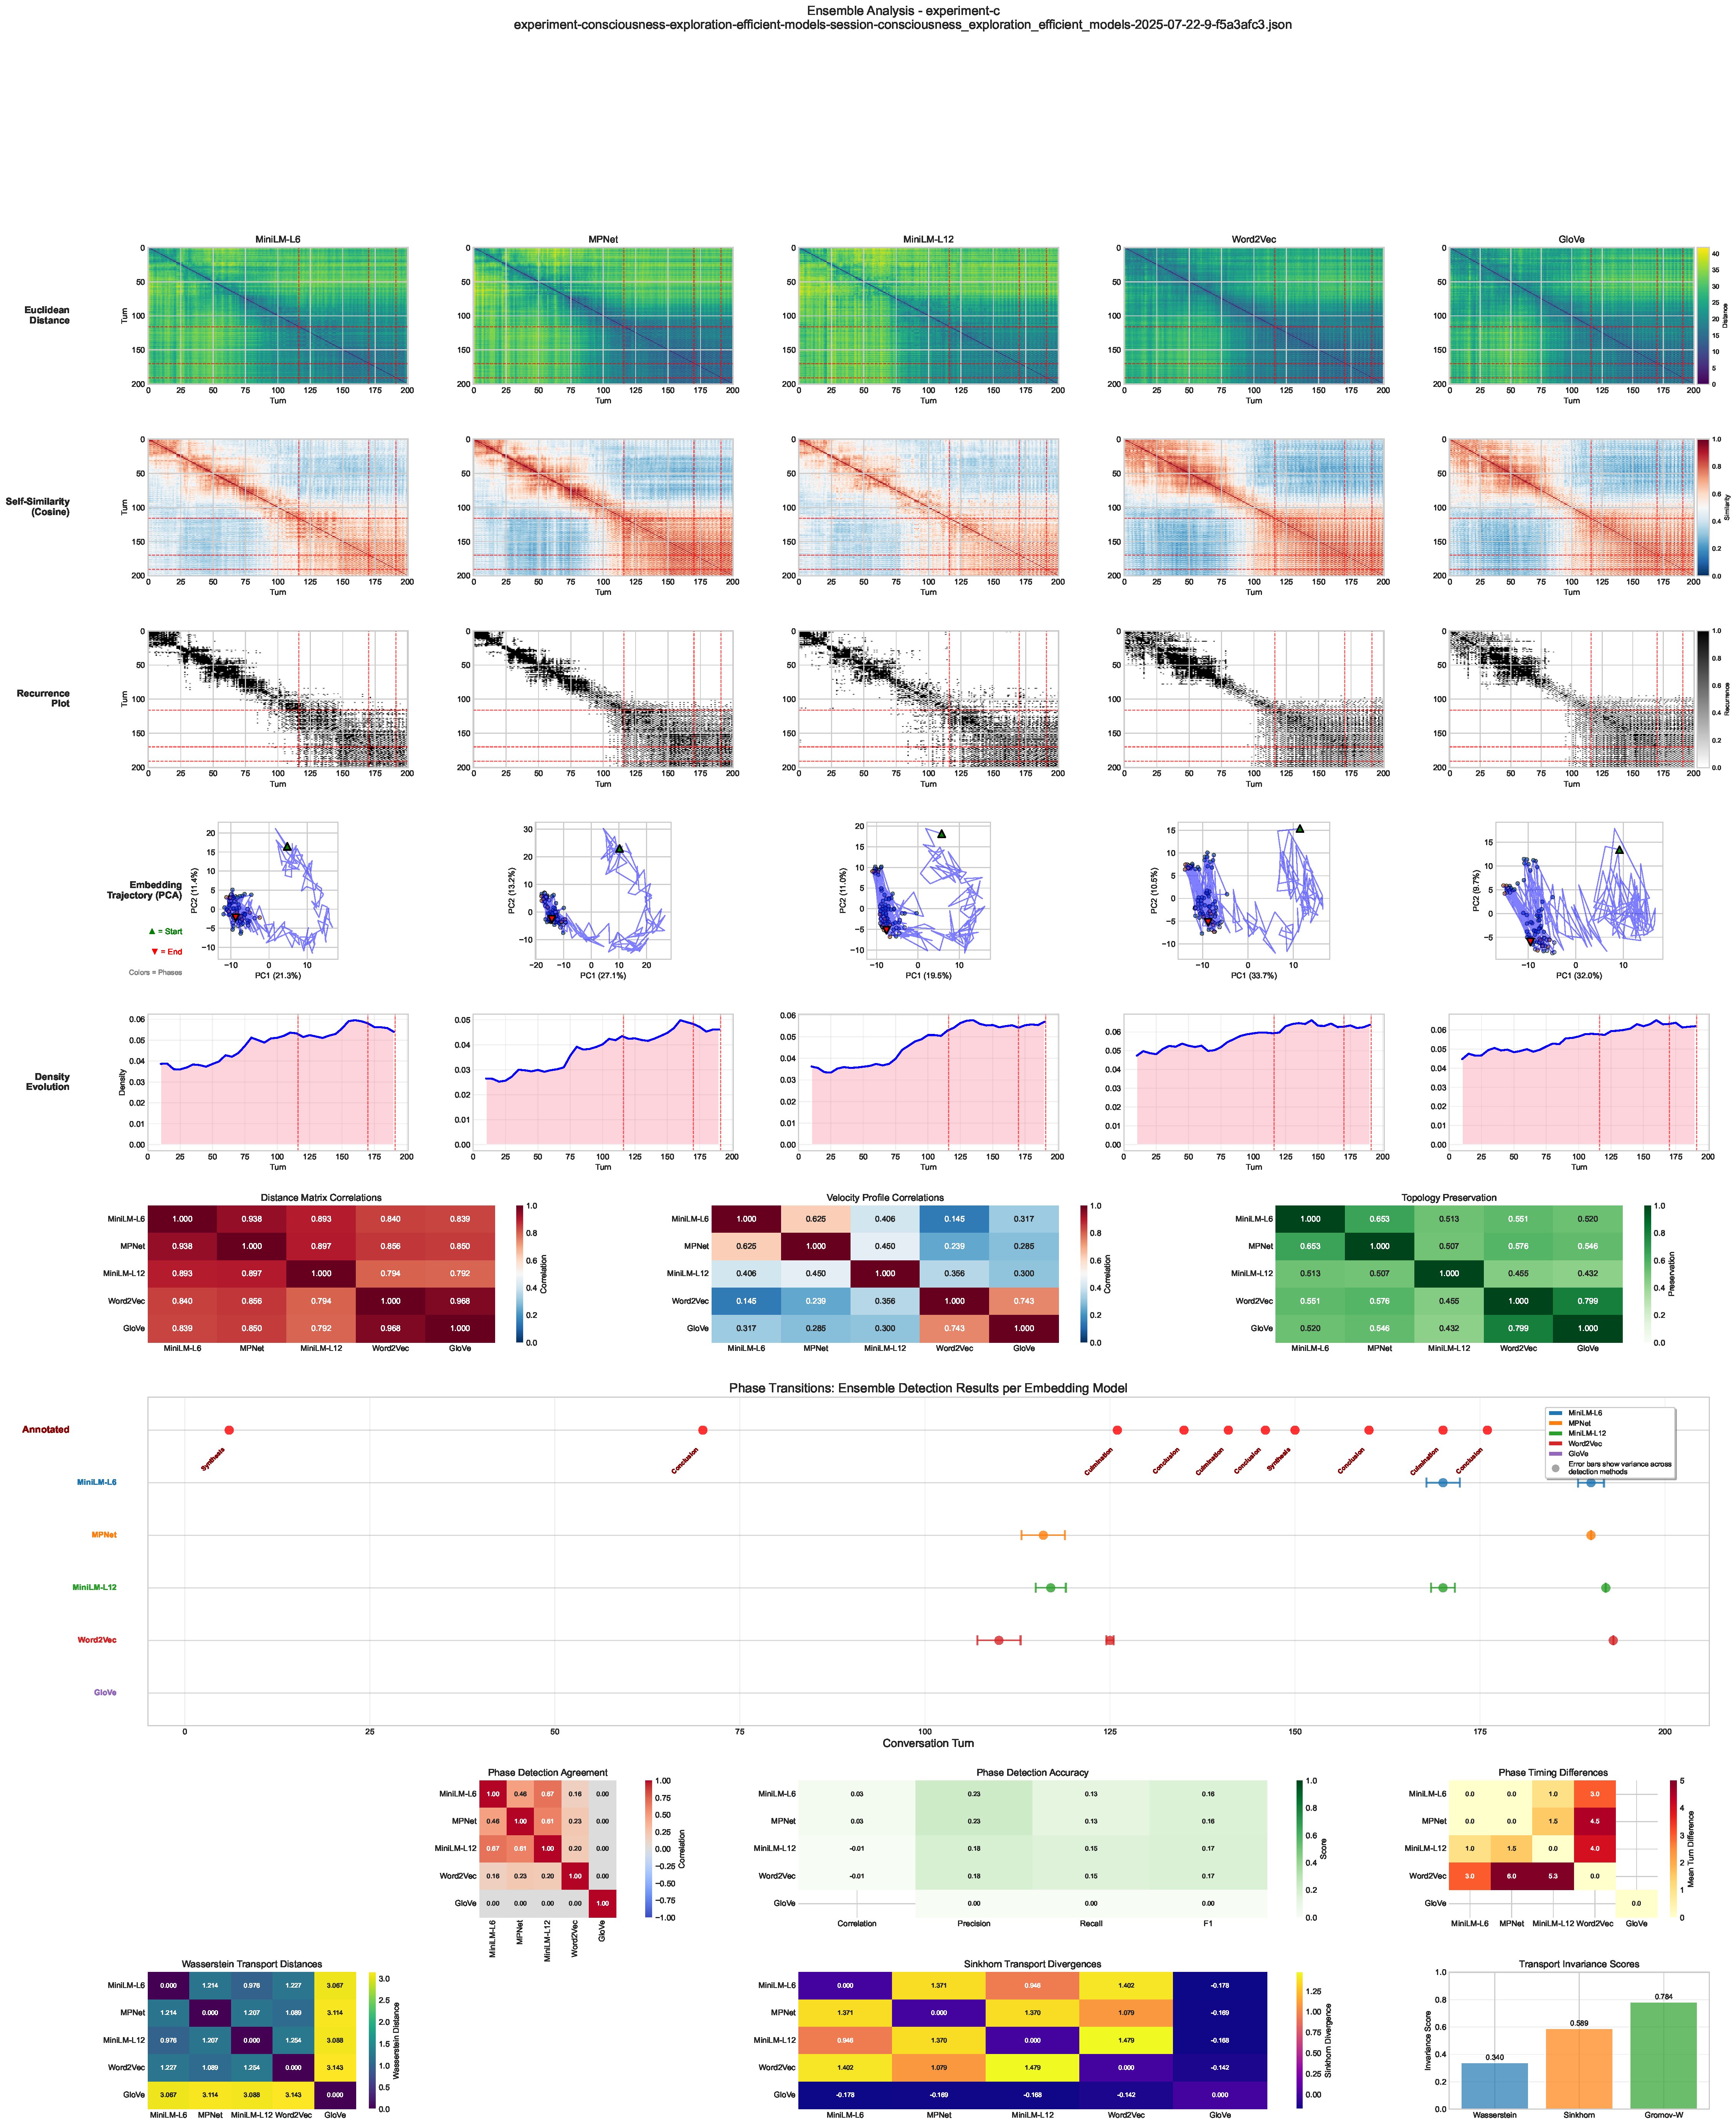
\includepdf[pages=1, pagecommand={\thispagestyle{plain}\label{fig:light_reasoning_1}}]{../analysis/analysis_output/figures/ensemble/pdf/experiment-consciousness-exploration-efficient-models-session-consciousness_exploration_efficient_models-2025-07-22-9-f5a3afc3_ensemble.pdf}
}

\afterpage{%
\clearpage
\thispagestyle{empty}
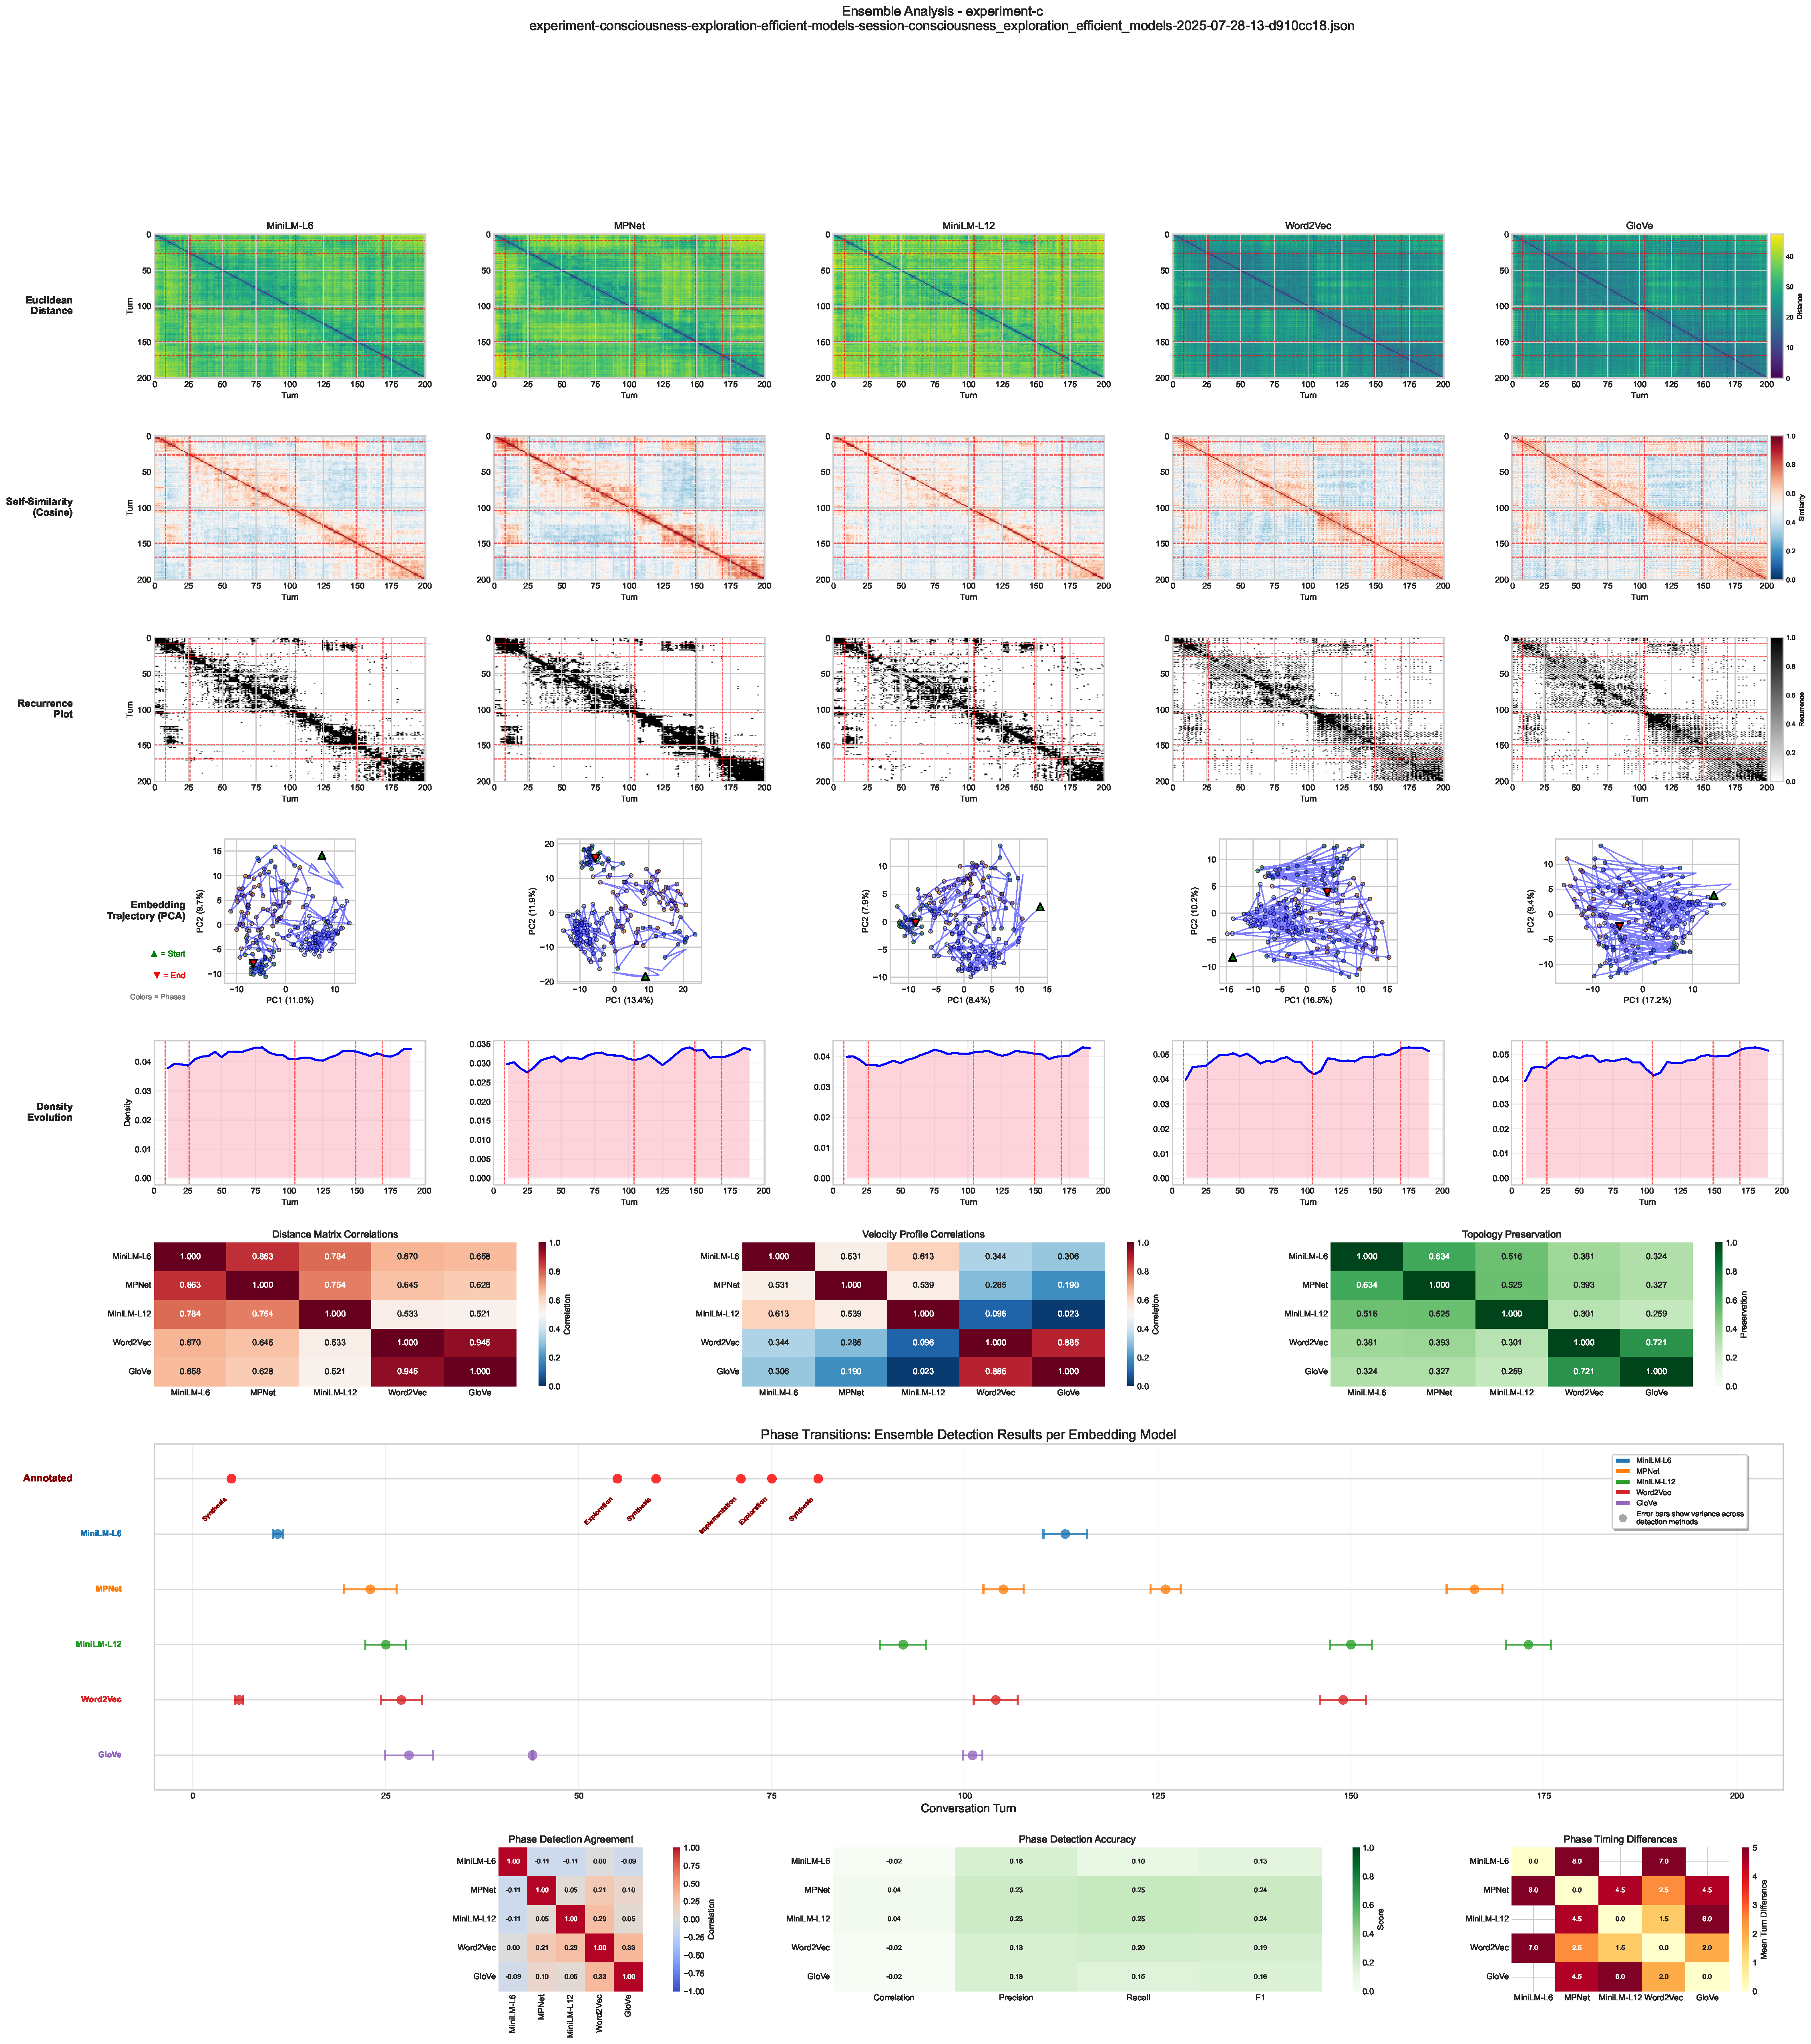
\includepdf[pages=1, pagecommand={\thispagestyle{plain}\label{fig:light_reasoning_2}}]{../analysis/analysis_output/figures/ensemble/pdf/experiment-consciousness-exploration-efficient-models-session-consciousness_exploration_efficient_models-2025-07-28-13-d910cc18_ensemble.pdf}
}

\afterpage{%
\clearpage
\thispagestyle{empty}
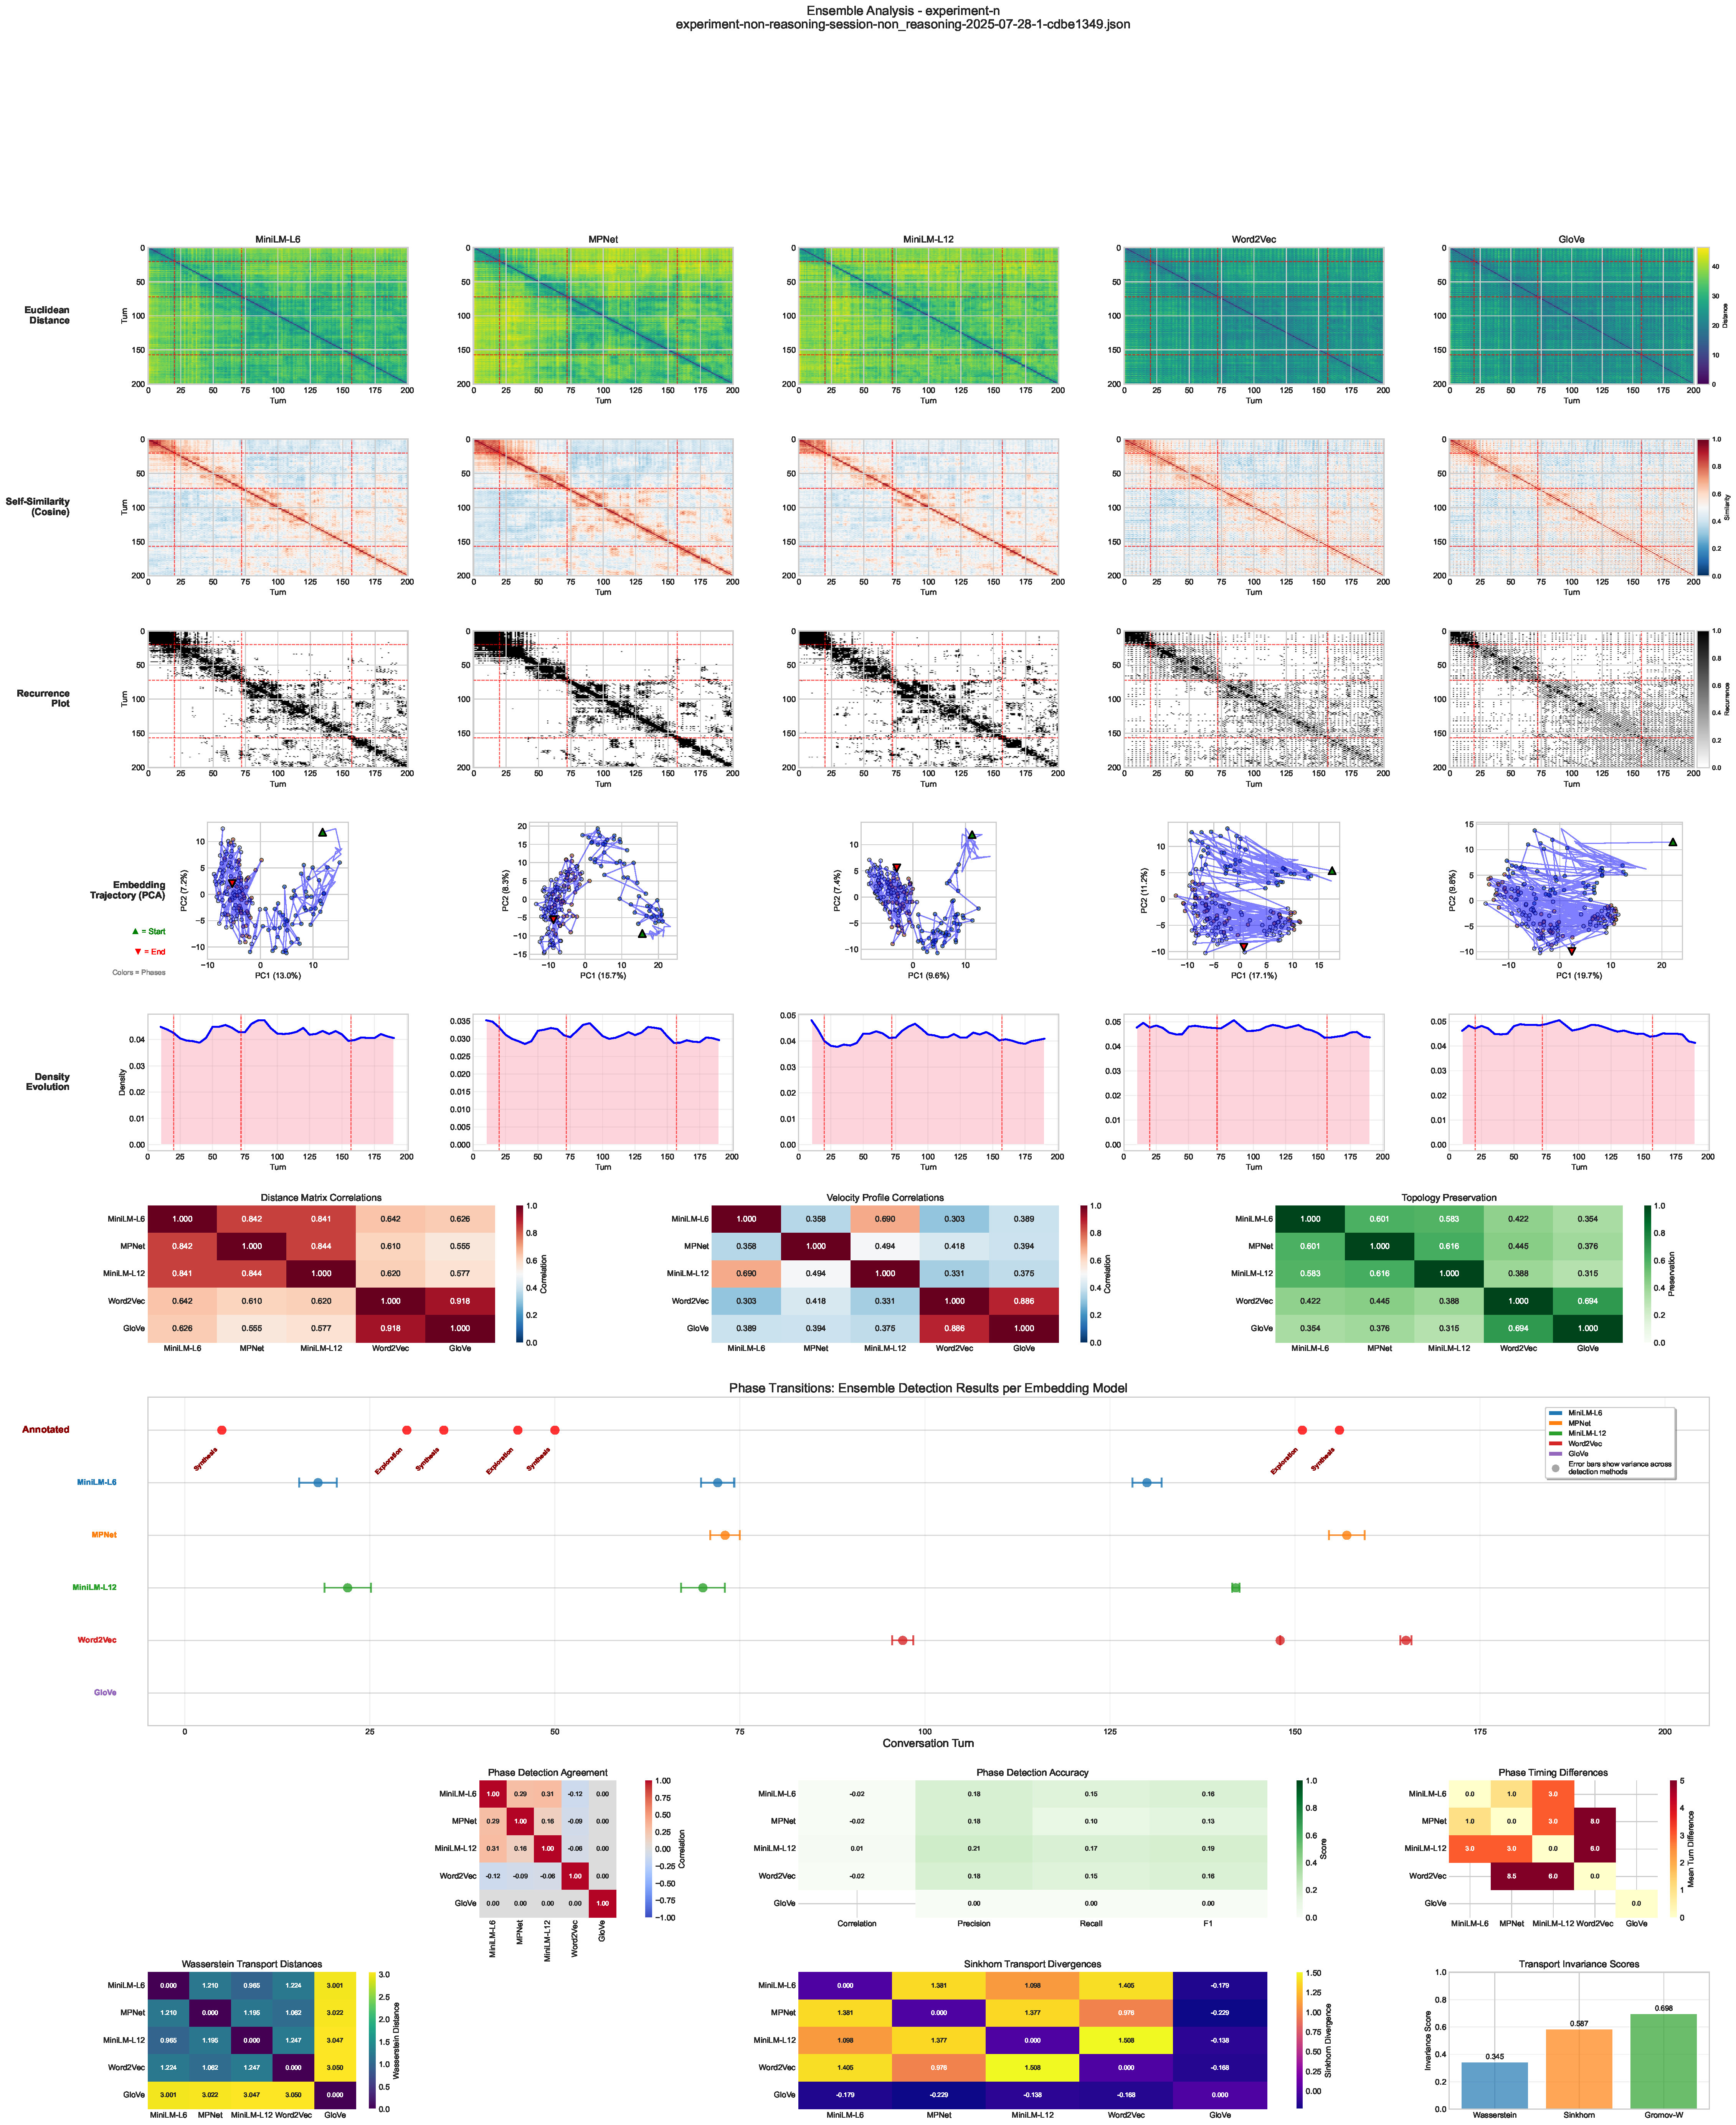
\includepdf[pages=1, pagecommand={\thispagestyle{plain}\label{fig:non_reasoning_1}}]{../analysis/analysis_output/figures/ensemble/pdf/experiment-non-reasoning-session-non_reasoning-2025-07-28-1-cdbe1349_ensemble.pdf}
}

\afterpage{%
\clearpage
\thispagestyle{empty}
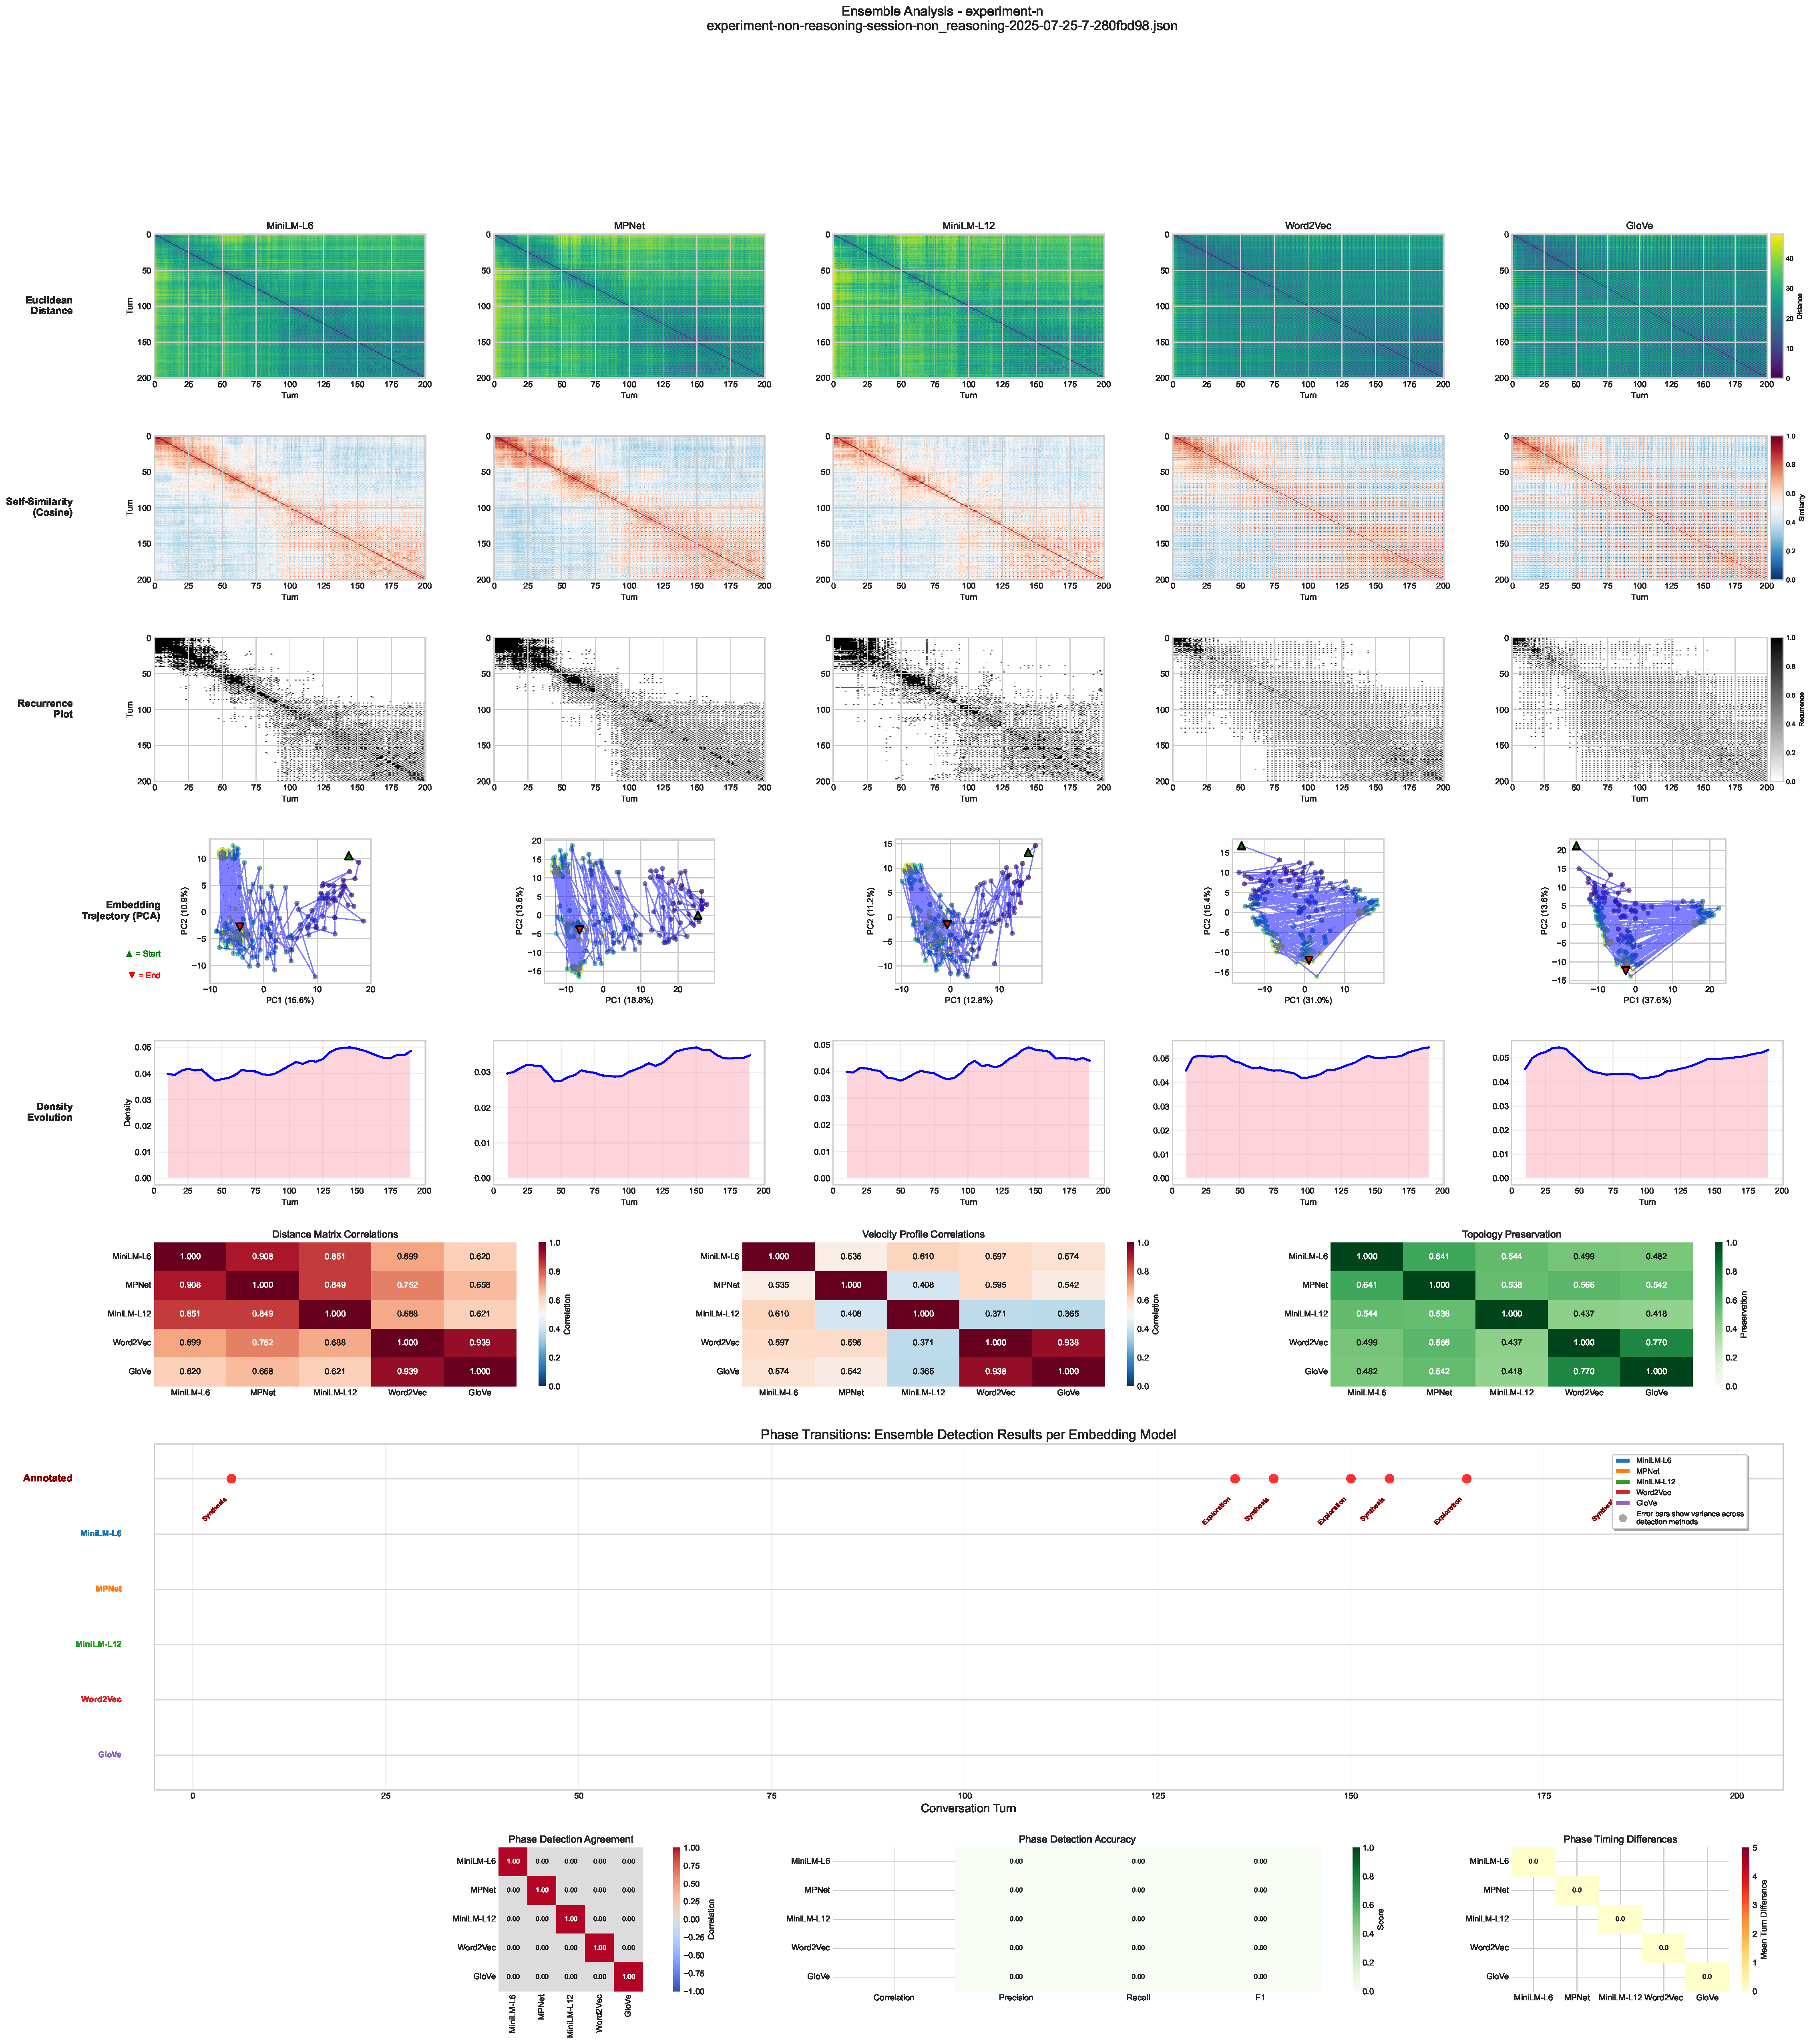
\includepdf[pages=1, pagecommand={\thispagestyle{plain}\label{fig:non_reasoning_2}}]{../analysis/analysis_output/figures/ensemble/pdf/experiment-non-reasoning-session-non_reasoning-2025-07-25-7-280fbd98_ensemble.pdf}
}

\end{document}